% **************************************************************************************************************
% A Classic Thesis Style
% An Homage to The Elements of Typographic Style
%
% Copyright (C) 2012 Andr\'e Miede http://www.miede.de
%
% If you like the style then I would appreciate a postcard. My address
% can be found in the file ClassicThesis.pdf. A collection of the
% postcards I received so far is available online at
% http://postcards.miede.de
%
% License:
% This program is free software; you can redistribute it and/or modify
% it under the terms of the GNU General Public License as published by
% the Free Software Foundation; either version 2 of the License, or
% (at your option) any later version.
%
% This program is distributed in the hope that it will be useful,
% but WITHOUT ANY WARRANTY; without even the implied warranty of
% MERCHANTABILITY or FITNESS FOR A PARTICULAR PURPOSE.  See the
% GNU General Public License for more details.
%
% You should have received a copy of the GNU General Public License
% along with this program; see the file COPYING.  If not, write to
% the Free Software Foundation, Inc., 59 Temple Place - Suite 330,
% Boston, MA 02111-1307, USA.
%
% **************************************************************************************************************
% Note:
%    * You must not use "u etc. in strings/commands that will be spaced out (use \"u or real umlauts instead)
%    * New enumeration (small caps): \begin{aenumerate} \end{aenumerate}
%    * For margin notes: \marginpar or \graffito{}
%    * Do not use bold fonts in this style, it is designed around them
%    * Use tables as in the examples
%    * See classicthesis-preamble.sty for useful commands
% **************************************************************************************************************
% To Do:
%		 * [high] Check this out: http://www.golatex.de/koma-script-warnung-in-verbindung-mit-listings-package-t2058.html
%    * [medium] mathbb in section-titles/chapter-titles => disappears somehow in headlines!!!
% **************************************************************************************************************
\documentclass[twoside,openright,titlepage,numbers=noenddot,headinclude=True,footinclude=True,parts,%1headlines,% letterpaper a4paper
                footinclude=true,cleardoublepage=empty,abstractoff, % <--- obsolete, remove (todo)
                BCOR=5mm,fontsize=11pt,english,%
                ]{scrbook}

\usepackage{libertine}

%********************************************************************
% Note: Make all your adjustments in here
%*******************************************************

\usepackage[utf8]{inputenc}
\usepackage{url}
\usepackage{microtype}
\usepackage{booktabs}
\usepackage{tabulary}
\usepackage{subcaption}
\usepackage{amstext}
\usepackage{rotating}
\usepackage{enumitem}
\usepackage{longtable}
\setlist{nolistsep}

% Fixing bug related to Pandoc to Latex conversion
\def\tightlist{}

% ****************************************************************************************************
% classicthesis-config.tex
% formerly known as loadpackages.sty, classicthesis-ldpkg.sty, and classicthesis-preamble.sty
% Use it at the beginning of your ClassicThesis.tex, or as a LaTeX Preamble
% in your ClassicThesis.{tex,lyx} with \input{classicthesis-config}
% ****************************************************************************************************
% If you like the classicthesis, then I would appreciate a postcard.
% My address can be found in the file ClassicThesis.pdf. A collection
% of the postcards I received so far is available online at
% http://postcards.miede.de
% ****************************************************************************************************

% ****************************************************************************************************
% 1. Configure classicthesis for your needs here, e.g., remove "drafting" below
% in order to deactivate the time-stamp on the pages
% ****************************************************************************************************
%\PassOptionsToPackage{eulerchapternumbers,listings,drafting,%
%				 pdfspacing,%floatperchapter,%linedheaders,%
%				 subfig,beramono,eulermath,parts}{classicthesis}
\PassOptionsToPackage{dottedtoc,listings,drafting,linedheaders,manychapters,pdfspacing,parts}{classicthesis}
% ********************************************************************
% Available options for classicthesis.sty
% (see ClassicThesis.pdf for more information):
% drafting
% parts nochapters linedheaders
% eulerchapternumbers beramono eulermath pdfspacing minionprospacing
% tocaligned dottedtoc manychapters
% listings floatperchapter subfig
% ********************************************************************

% ********************************************************************
% Triggers for this config
% ********************************************************************
\usepackage{ifthen}

% ****************************************************************************************************

% ********************************************************************
% Setup, finetuning, and useful commands
% ********************************************************************
\newcounter{dummy} % necessary for correct hyperlinks (to index, bib, etc.)
\newlength{\abcd} % for ab..z string length calculation
\providecommand{\mLyX}{L\kern-.1667em\lower.25em\hbox{Y}\kern-.125emX\@}
\newcommand{\ie}{i.\,e.}
\newcommand{\Ie}{I.\,e.}
\newcommand{\eg}{e.\,g.}
\newcommand{\Eg}{E.\,g.}
% ****************************************************************************************************


% ****************************************************************************************************
% 3. Loading some handy packages
% ****************************************************************************************************
% ********************************************************************
% Packages with options that might require adjustments
% ********************************************************************


\PassOptionsToPackage{english}{babel}   % change this to your language(s)
% Spanish languages need extra options in order to work with this template
%\PassOptionsToPackage{spanish,es-lcroman}{babel}
% \usepackage{babel}

\PassOptionsToPackage{fleqn}{amsmath}		% math environments and more by the AMS
 \usepackage{amsmath}

% ********************************************************************
% General useful packages
% ********************************************************************
\PassOptionsToPackage{T1}{fontenc} % T2A for cyrillics
	\usepackage{fontenc}
\usepackage{textcomp} % fix warning with missing font shapes
\usepackage{scrhack} % fix warnings when using KOMA with listings package
\usepackage{xspace} % to get the spacing after macros right
\usepackage{mparhack} % get marginpar right
\usepackage{fixltx2e} % fixes some LaTeX stuff
\PassOptionsToPackage{printonlyused,smaller}{acronym}
	\usepackage{acronym} % nice macros for handling all acronyms in the thesis

%\renewcommand*{\acsfont}[1]{\textssc{#1}} % for MinionPro
\newcommand{\bflabel}[1]{{#1}\hfill} % fix the list of acronyms


\usepackage{biblatex}
\bibliography{thesis}
\renewcommand\bibname{Bibliography}
% ****************************************************************************************************


% ****************************************************************************************************
% 4. Setup floats: tables, (sub)figures, and captions
% ****************************************************************************************************
\usepackage{tabularx} % better tables
	\setlength{\extrarowheight}{3pt} % increase table row height

\newcommand{\tableheadline}[1]{\multicolumn{1}{c}{\spacedlowsmallcaps{#1}}}
\newcommand{\myfloatalign}{\centering} % to be used with each float for alignment

\usepackage{caption}
\captionsetup{format=hang,font=small}
\usepackage{subcaption}
%\usepackage{subfig}
% ****************************************************************************************************


% ****************************************************************************************************
% 5. Setup code listings
% ****************************************************************************************************
\usepackage{listings}
\lstset{emph={trueIndex,root},emphstyle=\color{BlueViolet}}%\underbar} % for special keywords
\lstset{language=[LaTeX]Tex,%C++,
    keywordstyle=\color{RoyalBlue},%\bfseries,
    basicstyle=\small\ttfamily,
    %identifierstyle=\color{NavyBlue},
    commentstyle=\color{Green}\ttfamily,
    stringstyle=\rmfamily,
    numbers=none,%left,%
    numberstyle=\scriptsize,%\tiny
    stepnumber=5,
    numbersep=8pt,
    showstringspaces=false,
    breaklines=true,
    frameround=ftff,
    frame=single,
    belowcaptionskip=.75\baselineskip
    %frame=L
}
% ****************************************************************************************************


% ********************************************************************
% Using PDFLaTeX
% ********************************************************************
\PassOptionsToPackage{pdftex,hyperfootnotes=false,pdfpagelabels}{hyperref}
	\usepackage{hyperref}  % backref linktocpage pagebackref
\pdfcompresslevel=9
\pdfadjustspacing=1

\usepackage{graphicx}
\makeatletter
\def\maxwidth{\ifdim\Gin@nat@width>\linewidth\linewidth\else\Gin@nat@width\fi}
\def\maxheight{\ifdim\Gin@nat@height>\textheight\textheight\else\Gin@nat@height\fi}
\makeatother
% Scale images if necessary, so that they will not overflow the page
% margins by default, and it is still possible to overwrite the defaults
% using explicit options in \includegraphics[width, height, ...]{}
\setkeys{Gin}{width=\maxwidth,height=\maxheight,keepaspectratio}

% ********************************************************************
% Hyperreferences
% ********************************************************************
\hypersetup{
    %draft,	% = no hyperlinking at all (useful in b/w printouts)
    colorlinks=true, linktocpage=true, pdfstartpage=3, pdfstartview=FitV,%
    % uncomment the following line if you want to have black links (e.g., for printing)
    colorlinks=false, linktocpage=false, pdfborder={0 0 0}, pdfstartpage=3, pdfstartview=FitV,%
    breaklinks=true, pdfpagemode=UseNone, pageanchor=true, pdfpagemode=UseOutlines,%
    plainpages=false, bookmarksnumbered, bookmarksopen=true, bookmarksopenlevel=1,%
    hypertexnames=true, pdfhighlight=/O,%nesting=true,%frenchlinks,%
    urlcolor=webbrown, linkcolor=RoyalBlue, citecolor=webgreen, %pagecolor=RoyalBlue,%
    %urlcolor=Black, linkcolor=Black, citecolor=Black, %pagecolor=Black,%
    pdftitle={Rktik},%
    pdfauthor={\textcopyright\ Vincent Ahrend, University of Osnabrueck},%
    pdfsubject={},%
    pdfkeywords={},%
    pdfcreator={pdfLaTeX},%
    pdfproducer={LaTeX with hyperref and classicthesis}%
}
\urlstyle{same}  % don't use monospace font for urls


\setcounter{secnumdepth}{0}
% ********************************************************************
% Last, but not least...
% ********************************************************************
\usepackage{classicthesis}


\usepackage[a4paper,layout=a4paper]{geometry}

% ****************************************************************************************************


% ****************************************************************************************************
% 8. Further adjustments (experimental)
% ****************************************************************************************************
% ********************************************************************
% Changing the text area
% ********************************************************************
%\linespread{1.05} % a bit more for Palatino
%\areaset[current]{312pt}{761pt} % 686 (factor 2.2) + 33 head + 42 head \the\footskip
%\setlength{\marginparwidth}{7em}%
%\setlength{\marginparsep}{2em}%

% ***********************************

%********************************************************************
% Hyphenation
%*******************************************************
%\hyphenation{put special hyphenation here}

% ********************************************************************
% GO!GO!GO! MOVE IT!
%*******************************************************
\begin{document}
\frenchspacing
\raggedbottom
%\selectlanguage{american} % american ngerman
%\renewcommand*{\bibname}{new name}
%\setbibpreamble{}
\pagenumbering{roman}
\pagestyle{plain}
%********************************************************************
% Frontmatter
%*******************************************************

\begin{titlepage}
  \makeatletter
  \let\footnotesize\small
  \let\footnoterule\relax
  \let \footnote \thanks
  \null\vfil
  \begin{flushleft}%
        {\LARGE \sffamily Rktik \par}
    
    \vspace*{2cm}
        {\Large \sffamily A Social Network for Groups \par}%
    \vskip 2cm%
        {\large
     \lineskip .75em%
      \begin{tabular}[t]{c}%
       {\Huge Vincent Ahrend}
      \end{tabular}\par}%
      \rule{\linewidth}{1mm} \par
      \vskip 1cm%
    {\large BACHELOR'S THESIS 2015}\\[2cm]
    {\normalsize PRUEFER}\par
    {\large Dr. Helmar Gust, University of Osnabrueck \\ Dr. Kai-Uwe Kühnberger, University of Osnabrueck}  \par
    \vspace{3cm}
   \centering
    
\includegraphics[width=0.5\linewidth]{img/uos.png}
   \end{flushleft}\par
   \makeatother
\end{titlepage}

\pagestyle{scrheadings}





\pagestyle{scrheadings}



%\phantomsection
\refstepcounter{dummy}
\pdfbookmark[1]{\contentsname}{tableofcontents}
\setcounter{tocdepth}{2} % <-- 2 includes up to subsections in the ToC
\setcounter{secnumdepth}{3} % <-- 3 numbers up to subsubsections
\manualmark
\markboth{\spacedlowsmallcaps{\contentsname}}{\spacedlowsmallcaps{\contentsname}}
\tableofcontents
\automark[section]{chapter}

\renewcommand{\chaptermark}[1]{\markboth{\spacedlowsmallcaps{#1}}{\spacedlowsmallcaps{#1}}}
\renewcommand{\sectionmark}[1]{\markright{\thesection\enspace\spacedlowsmallcaps{#1}}}


\clearpage

\begingroup
    \let\clearpage\relax
    \let\cleardoublepage\relax
    \let\cleardoublepage\relax
    %*******************************************************
    % List of Figures
    %*******************************************************
    %\phantomsection
    \refstepcounter{dummy}
    %\addcontentsline{toc}{chapter}{\listfigurename}
    \pdfbookmark[1]{\listfigurename}{lof}
    \listoffigures

    \vspace*{8ex}

    
%   \newpage

    

\endgroup

\cleardoublepage


\pagenumbering{arabic}
%\setcounter{page}{90}
% use \cleardoublepage here to avoid problems with pdfbookmark
\cleardoublepage

\chapter{Introduction}\label{introduction}

Rktik\footnote{The project's name is neologism that is reminiscent of
  the German ``Arktis'' and English ``Arctic''. It was chosen because it
  allows for a short domain name (\url{rktik.com}). Additionally, the
  connection to the Arctic, seafaring, and related concepts offer a
  variety of options for branding Rktik.} is an online community that
allows like-minded people to collect and publish content together. Rktik
is set apart from similar online services by its distinct modelling of
individual user and group identity. This thesis describes Rktik's
software architecture and how it fulfills its development goals. The
first chapter motivates the project and gives an introduction to
methodology and comparable products. Then a conceptual description of
Rktik's functionality is given. Following that, the technical background
of implementation and operation of the service is described. The last
chapter contains an evaluation and discussion of the project and its
future development.

\hyperdef{}{motivation}{\section{Motivation}\label{motivation}}

Rktik is the successor to the Souma app, which started as a hobby
project of Vincent Ahrend in 2012 and was then developed from 2013-2014
in the Cognitive Networks study project at University of Osnabrück
(CITE). Souma's original motivation was the sharing of files with groups
of friends in a service with a modern user interface that does not rely
on the benevolence of central service providers. Over the course of
development however, the goals of this project changed significantly.

At first the aim was to combine social networking functionality with
filesharing tools. This functionality can only be provided by a
decentralized system due to privacy and legal reasons. The
\emph{Cognitive Networks} study project developed this idea further and
priorities shifted to a focus on the more general goal of a
\emph{humanist social platform}. Such a platform would not place
economic constraints and existing metaphors for social software systems
at the center of its conceptualization, but instead develop solutions
from the ideals of humanism.

This shift in the goals of the study project, combined with the remnants
of various side projects embedded in the app obscured the core of the
project in the code base of Souma. Therefore, after the end of the study
project, Rktik was conceptualized as a new web-based platform based on
the server-side component of Souma. It has now a much more limited
focus: Developing a social publishing platform that implements a new
concept of individual and group identity online. This will allow users
to forge new online identities that they can use to evade the now
all-encompassing surveillance of online activities by corporations and
government agencies. Sorted by priority, the goals of this process are:

\begin{enumerate}
\def\labelenumi{\arabic{enumi}.}
\tightlist
\item
  Bringing the application from prototype status to being ready and
  useful for end users by implementing a complete feature set
  (\textbf{completeness})
\item
  Selecting the smallest set of features that allows users an efficient
  management of privacy and can be implemented by a single developer
  (\textbf{feasibility})
\item
  Stripping out and refactoring code from the Souma prototype that is no
  longer required in Rktik in order to make the project maintainable in
  the future (\textbf{maintainability})
\end{enumerate}

\hyperdef{}{problem-privacy-and-identity}{\section{Problem: Privacy and
Identity}\label{problem-privacy-and-identity}}

The essential problem in managing privacy in online systems is the need
of service providers to directly access user data. This need exists for
both, cloud-based web applications, as well as native
applications\footnote{Native applications are run on the user's local
  machine and stand in contrast to web applications which are run on a
  server and present their user interface as a web site.} that offload
parts of their data processing to remote servers (which is the case for
many native mobile applications). Companies need direct access to user
data, in order to take advantage of central data processing facilities
running on web servers. Some of the advantages of web applications, as
opposed to native applications without a remote backend, are: 1) no
software piracy, 2) more efficient maintenance due to direct access to
the running system, and 3) no need to support a wide range of (possibly
low-performance) user hardware.

Besides the need of service providers to access user data, government
agencies are also surveilling large parts of online communications.
While the power of large organizations to access user data is still not
fully understood, it can be assumed that accessing unencrypted user data
that is directly bound to a real name presents the lowest barriers to
access. This wide-spread surveillance from multiple fronts stands in
stark contrast to the availability of end-user tools for shaping their
online privacy and identity.

One possible solution is presented in the proposed peer-to-peer
extension of Rktik (see \hyperref[external-clients]{External Clients}).
It would approach this problem directly by using cloud infrastructure
for transferring data, while processing and storing data on user
machines. While this solution does not come with the mentioned
advantages of web applications, it offers a lot of value to users who
place importance on their privacy. Due to the technical complexity of
implementing a peer-to-peer protocol, a second solution to the problem
was developed.

The approach pursued in this thesis offers users increased control over
their privacy by partially decoupling their offline identity from what
they do online. This is achieved by extending the concept of
pseudonymity in letting 1) a single person control multiple pseudonyms
and 2) letting multiple persons control a shared pseudonym.

\hyperdef{}{methodology}{\section{Methodology}\label{methodology}}

The Rktik application is based on the Souma prototype developed in the
Cognitive Networks study project (see Ahrend (2015)). In line with the
goals outlined in \hyperref[motivation]{Motivation}, Rtkik's development
process included

\begin{enumerate}
\def\labelenumi{\arabic{enumi}.}
\tightlist
\item
  Defining required functionality
\item
  Setting up a development environment
\item
  Implementing features
\item
  Setting up third-party infrastructure
\item
  Finding and removing bugs
\item
  Evaluation
\end{enumerate}

The Github issue tracker\footnote{Access to the issue tracker is
  restricted to Github accounts registered as Rktik developers. See
  \href{https://github.com/features}{Github Features}} was used to
record these tasks and eventual subtasks. A Git repository, also hosted
on Github, was used to track the contents of the source code. Changes in
the source code are referenced from the issue tracker when they are
connected to the resolution of an issue. Using Git and Github helps to
keep an overview of tasks and their relation to specific source code
changes and offers quick access to past versions of the source code.
This feature can be valuable as it allows deleting code without worrying
that it might still be needed later on in development.

The Rktik application is implemented in the Python programming language,
using the Flask framework for web applications and the SQLAlchemy object
relational mapper. Additionally, some features of the user interface are
implemented using the jQuery library. The operating environment is
provided by Heroku in the form of a platform-as-a-service (PAAS). A PAAS
allows uploading and running a web application on provisioned servers
without having to configure these servers manually. See
\hyperref[hosting-and-deployment]{Hosting and Deployment} for more
details on this process.

These choices were taken from the Souma project which used the same
technological stack.

\hyperdef{}{state-of-the-art}{\section{State of the
Art}\label{state-of-the-art}}

This section describes approaches to social networks that share
similarities with Rktik. I will explain their functionality and
specifically focus on their representation of identity and related
software features.

This comparison includes three social platforms with more than 100
million monthly active users, each of which has a bias towards a
different communication structure. This includes Facebook as a social
network used for communication within \emph{peer-groups}, Reddit as an
open social network where users publish to the \emph{general public} and
email as a communication medium used for \emph{direct communication}
with other users. All three services can also be used for one-to-one,
one-to-many and many-to-many communication.

In the following, I will explain the basic functionality of each of the
services and then compare them to Rktik.

\textbf{Facebook}

Available since: February 2004\\
Monthly active users: 1.49 billion as of June 30, 2015 ((Facebook,
n.d.-b))\\
Website: \href{http://facebook.com/}{facebook.com}

Facebook is an online social networking service, it allows friends and
acquaintances to keep track of each other's personal lifes. Facebook
offers a similar core functionality to that of Rktik in that users can
publish content on their profiles, vote\footnote{Votes on Facebook are
  called ``like''.} and comment on content of other users and subscribe
to their content feeds. Both services center the user interface on a
feed of content from subscribed sources that is sorted based on a
combination of recency and other factors. Facebook also allows users to
create groups as either public or private spaces. Members can then
communicate in a group chat or post messages to the group's feed.
Messages can contain events, votes and files/media.\footnote{Files must
  not be music or executables and their file size cannot exceed 25mb.}
Users may also communicate via private messages.

In contrast to these similarities, Facebook is different from Rktik both
in policy and features. It requires users to identify with their real
name and explicitly forbids creating more than one personal user account
((Facebook, n.d.-a)). Contents of the Facebook network are hidden from
the public by default and accessible only once a friendship connection
has been established with a user. Facebook groups can only choose to be
either public or private. In contrast to Rktik, private groups cannot
publish contents publicly and groups in general cannot publish content
in the name of the group.

In addition to the core and group functionality, Facebook offers many
features ranging from business directories to video calling. These have
not been included in this comparison as they do not directly compare to
features of Rktik.

\textbf{Reddit}

Available since: June 2005\\
Monthly active users: 203 million as of September 15, 2015 (Reddit
(n.d.-a))\\
Website: \href{https://reddit.com}{reddit.com}

Reddit is a social link aggregator, it lets users create link and text
submissions and sorts them based on user votes and recency. Submissions
are created in \emph{subreddits}, which are subcommunities of Reddit
related to a specific topic. Each submission has a comments section in
which its contents are discussed by the community. Comments can also be
voted on and are displayed in a hierarchical layout based on their
reply-structure. Each subtree is sorted according to number of votes and
recency.

Users of reddit can collect \emph{karma}, which is a numeric value that
is displayed on their profile and indicates the amount of votes they
have received on their own comments and submissions.

This core functionality of Reddit is mostly identical to that of Rktik.
Differences between the services can be found in their implementation of
user and group identity as well as the way external contents are
displayed.

In contrast to Facebook, Reddit encourages the creation of multiple
accounts per user (Reddit (n.d.-b)). However, it does not provide user
interface controls for this. Every account is identified by its
username, which is pseudonymous and does not necessarily reflect the
real identity of a user in any way.

Users can not directly publish content on a user profile or blog, as all
submissions must be placed in one of Reddit's communities, which are
called \emph{Subreddits}. They allow the aggregation of content related
to a specific topic. Their contents are visible either for the general
public or only for confirmed members, as decided by the subreddit's
founding user. In contrast to Rktik, Reddit does not allow subreddits to
aggregate content in a space visible only to members, while also
publishing content in a public space.

The content on reddit.com is almost text-only. If a link submission
points at an image, a small preview is displayed next to the
submission's title, while links to other content are never rendered
inline.

\textbf{Email}

Available since: \textasciitilde{} 1971\footnote{As the email protocol
  evolved over time from non-networked messaging protocols, there is no
  specific point in time from which on email was generally available. In
  1971 the first networked electronic mail system for ARPANET was
  standardized (@{[}Crocker1982{]}).}\\
Monthly active users: \textgreater{} 2 billion\footnote{It is difficult
  to estimate the number of people who actively use email because of the
  large number of email service providers. The market research firm
  Radicati estimated a number of 2.6 billion active email users in 2015
  (Radicati \& Hoang (2011)).}\\
Website: none

Email is a protocol for distributing messages from an author to one or
many recipients. While Rktik, Facebook and Reddit are offered by their
respective providers, Email is a \emph{method} of message delivery that
is implemented by many service providers worldwide, while still allowing
all users to exchange messages with each other. Email messages may also
contain any number of media attachments.

A user of Email is identified by their email address. Some email service
providers let users choose a username for themselves, while others have
policies regarding usage of a real name or other personally identifying
features, such as their role in a company. As there is no single user
interface for email, users can chose from a wide range of software
clients. These can be websites, dedicated email applications, or email
features embedded in other applications. Available features depend
entirely on the client used.

Email can be used in combination with \emph{automated email lists} for
similar use cases as those Rktik was designed for. Automated email
lists, or \emph{email lists}, are distribution services that forward
incoming messages, sent to a special email address, to all users
registered with the email list. Registration may be open to the general
public or restricted to a group of users defined by the email list
operator. Messages sent to the email list may also be read using a web
based discussion archive.

An email list is similar to Rktik movements, subreddits and Facebook
groups in that it provides members with a space for discussion and
exchange related to a specific topic. Submissions are tied to their
author and discussion may be hierarchically organized by reply-structure
as is the case in Reddit and Rktik. Email does not provide a mechanism
for voting on messages, so discussions are sorted chronologically. Email
lists also do not offer features for collectively authoring content and
publishing it to people outside the email list.

\begin{longtable}[c]{@{}lll@{}}
\caption{Overview of username restrictions and group
features}\tabularnewline
\toprule
Platform & Username & Group Features\tabularnewline
\midrule
\endfirsthead
\toprule
Platform & Username & Group Features\tabularnewline
\midrule
\endhead
Facebook & Real name & Discussion, voting, group chat, events, file
sharing\tabularnewline
Reddit & Pseudonym & Discussion\tabularnewline
Email & Both & Discussion, file sharing\footnote{File sharing may be
  prohibited by the email list operator.}\tabularnewline
Rktik & Pseudonym & Discussion, group chat, publishing\tabularnewline
\bottomrule
\end{longtable}

In conclusion, Rktik as a social platform has many similarities to
existing social platforms. Established concepts and functionality such
as user profiles, private messaging, media attachments and others are
extended with a novel conceptualization of personal and group identity.
These new features extend user's capabilities in shaping their privacy.
New group functionality may serve as a catalyst to processes defining
the group's online identity. Other platforms, especially Facebook, also
offer extended group features, but are not considering groups as an
identity that can publish content itself.

\chapter{Conceptual}\label{conceptual}

\section{Overview}\label{overview}

Rktik is an online community where users share text, links and other
media pseudonymously in the context of topic-oriented groups and
personal blogs. Contents are sorted based both on recency as well as a
voting and subscription system.

This chapter will explain the user-facing functionality of the Rktik
website on a conceptual level. First, general concepts are explained,
introducing readers to the mechanics of using Rktik. Subsequent sections
give detailed information on how Rktik handles \emph{content},
\emph{identity} and \emph{context}.

\hyperdef{}{terminology}{\subsection{Terminology}\label{terminology}}

This section gives a brief overview of terminology used in Rktik. Please
see the relevant subsequent sections for more in-depth descriptions.

\textbf{Users} are individual persons using the site. They may register
by creating a \emph{user account} and one or more associated
\emph{personas}. Hereby they are able to create content on the site.

(see \hyperref[user-accounts]{User Accounts})

All actions of users are attributed to their \textbf{active persona},
which is a screen name that identifies them across the site. A user may
create any number of personas to shape their privacy, but only one of
them can be \emph{active} at a time.

\textbf{Thoughts} are short pieces of text submitted by personas and
represent the smallest unit of content.

(see \hyperref[overview-thoughts]{Overview: Thoughts})

Thoughts can link to any number of \textbf{percepts}, which are
attachments containing either more text or a hyperlink to an external
resource. They are displayed alongside the thought throughout the user
interface.

(see \hyperref[attaching-media-percepts]{Attaching Media: Percepts})

Personas can \textbf{vote} on thoughts to make them more visible to
other users. Every thought has a numerical \textbf{hotness} value, which
decreases with time after posting and increases with every vote gained.
This value is used for sorting many thought listings.

(see \hyperref[hotness]{Distributing Attention: Voting and Hotness})

\textbf{Mindsets} are collections of thoughts. Any thought that is not a
reply to another thought must be contained in a mindset. Every persona
has a private and a public mindset (\textbf{notebook} and \textbf{blog}
respectively).

(see \hyperref[context]{Context})

\textbf{Movements} are groups related to a specific topic. Each of them
has a private mindset for members and a public mindset (blog).

Any persona can create new movements and follow the (public) blog of any
movement or other persona.

(see \hyperref[movements]{Movements})

See \hyperref[nucleus-models]{Nucleus Models} for a diagram showing the
relation of these concepts in Rktik.

\subsection{Frontpage}\label{frontpage}

The \emph{frontpage} is located at the root of Rktik and presents users
with a stream of thoughts from their movements and followed blogs. It is
similar to the \emph{Facebook News Feed} and the \emph{Reddit frontpage}
in that the stream is sorted based both on the recency of a submission
and the number of votes it has received (see
\hyperref[hotness]{Distributing Attention: Voting and Hotness}).

Anonymous users do not have any subscriptions, they are shown thoughts
from \emph{top movements}. These are the seven movements with the
highest member count.

On the right-hand side of the thought stream, the frontpage also
contains a number of other elements:

\begin{itemize}
\tightlist
\item
  The \textbf{frontpage graph visualization}: A visual representation of
  all thoughts and authors on the page as a graph (see
  \href{img/graph.png}{Frontpage Graph Visualization}).
\item
  \textbf{Top Thought}: When a user is logged in, this contains a short
  list of thoughts from \emph{top movements} they are not following with
  their active persona. This allows users to notice particularly popular
  submissions from contexts they would not see otherwise.
\item
  \textbf{Discover Movements}: A listing of those top movements the
  active persona is not following.
\item
  \textbf{Recent Thoughts}: The most recent publicly visible thoughts
  submitted throughout the whole site.
\end{itemize}

\subsubsection{Frontpage Graph
Visualization}\label{frontpage-graph-visualization}

\begin{figure}[htbp]
\centering
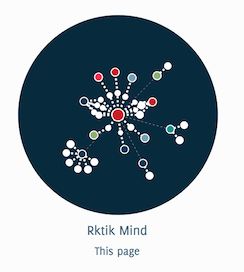
\includegraphics{img/graph.png}
\caption{Frontpage graph visualization}
\end{figure}

The frontpage contains a visual representation of its contents in the
form of a graph with a force-directed layout. This layout communicates
the flow of information from a persona's subscriptions to their
frontpage. It also shows some additional thoughts from these
subscriptions, that are not \emph{hot} enough to be included in the
frontpage.

The graph represents the frontpage as a big red node in the center,
identities which are followed by the active persona (content sources) as
medium-sized colored nodes and thoughts as small white nodes.

Thoughts are connected to the center node with a dotted edge if they are
currently part of the frontpage feed. Thoughts are also always connected
to their author's identity with a further dotted edge. Some of the
identities followed by the active persona may have contributed no
thoughts to the current frontpage. In this case, they are connected to
the center with a faint dashed edge. Nodes representing thoughts have a
pulsating animation with a frequency correlated to their hotness and
capped at 5 Hz.

Thereby, the frontpage contents surround the center node as a ring of
white nodes, pulsating faster or slower according to their position in
the stream. They are connected to a second ring of nodes which consists
of those movements and personas who submitted the thoughts. Other
content sources are located a bit further away to show that their
submissions are also eligible for inclusion in the frontpage.

\subsection{Notifications}\label{notifications}

Notifications catch the user's attention in order to present information
which is personally relevant. They are displayed in a drop down menu in
the top left corner of every page and some of them are also sent as
email notifications.\footnote{A user may opt out of receiving emails
  about notifications of a specific type. See
  \hyperref[user-accounts]{User Accounts}.}

\begin{figure}[htbp]
\centering

\includegraphics{img/notifications.png}
\caption{Notification menu showing one unread notification about a
received private message}
\end{figure}

There are four notification types:

\begin{itemize}
\tightlist
\item
  \textbf{Reply}: Sent when another user replies to one of the active
  user's thoughts
\item
  \textbf{Mention}: Sent when someone uses the
  \emph{@\textless{}username\textgreater{}} syntax in a thought to
  notify a persona directly.
\item
  \textbf{Dialogue}: Sent when a new thought is added in a private
  conversation
\item
  \textbf{Follower}: Sent when a persona's Blog gains new followers
\end{itemize}

See \hyperref[notification]{Notification} for implementation details.

\section{Content}\label{content}

\hyperdef{}{overview-thoughts}{\subsection{Overview:
Thoughts}\label{overview-thoughts}}

\emph{Thoughts} are the basic building block for content in Rktik and
roughly equivalent to a post on Facebook or submission on Reddit. They
consist of a short text, limited to 300 characters, and any number of
percepts (attachments). Thoughts are displayed 1) as part of blogs and
mindspaces, 2) on individual thought pages or 3) as part of a chat
conversation (see \hyperref[context]{Context}).

The restriction on title length has been set for two reasons:

\begin{enumerate}
\def\labelenumi{\arabic{enumi}.}
\tightlist
\item
  Page layouts can be simpler. Longer titles lead to a bigger variation
  in title length, which would make the usage of separate display styles
  for long and short titles necessary. Implementing these increases
  development and maintenance time.
\item
  Short titles require users to be concise when formulating thoughts. In
  turn, they make it easier for other users to read and understand
  titles.
\end{enumerate}

Thoughts can be created using the dedicated \emph{create thought} page
or the \emph{inline thought creator}. All mindsets in which the active
persona has editing rights contain a link to the create thought page.
The inline thought creator is embedded in comments sections and as part
of the chat widget. It only allows posting text content up to the length
of a thought's title (300 characters), but lets users switch to the
create thought page without losing their input if they wish to continue
typing. The dedicated create thought page provides separate input fields
for title and longform text attachments.

\hyperdef{}{reposts}{\subsection{Reposts}\label{reposts}}

Thoughts can be \emph{reposted}, which creates a copy of the original
thought, but links it to a different mindset and attributes it to the
persona who created the repost. Reposts are always created as comments
on their original, thereby notifying the original author. Visiting a
repost's page, users see the original thought from which it was created
displayed in the context area.

\hyperdef{}{attaching-media-percepts}{\subsection{Attaching Media:
Percepts}\label{attaching-media-percepts}}

Thoughts may have any number of attachments to enrich their content.
These are either rendered as part of the Rktik website or presented as
links to other websites.

Currently the following attachment kinds are supported:

\begin{itemize}
\item
  \textbf{Link}: This type can be attached by embedding a URL inside the
  thought title or longform text.

  Links to pictures may be rendered inline with the thought. Clicking
  the picture displays it enlarged in a modal gallery view. If multiple
  links to pictures are linked to a single thought, the modal view
  allows browsing through the picture gallery using keyboard and
  onscreen controls. The display size of pictures is also adapted to the
  size and number of image attachments (see
  \hyperref[html-templates]{HTML Templates}).

  Links that point to the \emph{soundcloud.com} and \emph{youtube.com}
  domain will be rendered using the respective embeddable widgets to
  allow playing music and videos without leaving the Rktik website.
\item
  \textbf{Longform text} As thought titles are limited to 300
  characters, the longform text attachment allows adding a longer text.
  This text may be formatted using Markdown syntax ((Gruber, 2004)),
  which provides simple markup for basic text formatting such as
  headlines, enumerations, bold and italic text.
\end{itemize}

\hyperdef{}{hotness}{\subsection{Distributing Attention: Voting and
Hotness}\label{hotness}}

Personas may vote on thoughts, thereby expressing approval of their
content. The number of votes is displayed next to every thought.

Apart from being a visible signal about the number of people who have
expressed approval of a thought, votes are also used for sorting
thoughts in the hotness sorting algorithm (see
\hyperref[hotness]{Distributing Attention: Voting and Hotness}).
Depending on context, the order of thoughts is either chronological
(chat), reverse chronological (blog) or by their \emph{hotness} value.

Hotness is a numeric value which depends on the recency of a thought and
the number of votes it has received. Accordingly, hotness values are
higher for more recent thoughts or thoughts with more votes. Thoughts
with equal numbers of votes are effectively sorted in reverse
chronological order, while each additional vote pushes the thought
upward in the ordering.

Given the number of upvotes (v) and the number of hours since the
thought was created (t), a thought's hotness is:

\begin{verbatim}
hot = v / pow(t + 2, 1.5)
\end{verbatim}

This algorithm is adapted from the sorting algorithm used in the social
bookmarking site \href{https://news.ycombinator.com/}{Hacker News} (see
(Salihefendic, 2010)).

\section{Identity}\label{identity}

Some popular social media sites including Google+ and Facebook have
tried to push users into publishing content on their services using a
real name ((Boyd, 2012)). The practice proved to be controversial, as it
did not align with established Internet culture and prevented people
from decoupling their online and offline activities (CITE).

However, even though a pseudonymous naming system prevents directly
linking offline and online identity based on metadata, such a link can
be established by other means. Content posted online may be uniquely
bound to an offline identity or link to other online contents that
establish such a binding.

Rktik introduces new tools that allow users to shape their digital
privacy. Every user may create multiple online identities and use them
to separate areas of their online activity. Users may also join their
identities by publishing under the name of a movement. The following
section will explain these concepts in detail.

\hyperdef{}{user-accounts}{\subsection{User
Accounts}\label{user-accounts}}

Any user of Rktik can register a personal user account which allows them
to create content and vote on submissions. Creating an account requires
a valid email address, a password and a name and color value for the
user's first persona. The color value is used for decorative purposes in
the site's design.

The account feature serves two main purposes:

\begin{enumerate}
\def\labelenumi{\arabic{enumi}.}
\tightlist
\item
  Authorizing a user's identity by asking them to enter the
  account-specific password and email-address combination. Authorized
  users may act on the site as one of the personas connected to the user
  account.
\item
  Obtaining a valid email address so that users may be sent
  notifications and other messages related to their activity on the
  site.
\end{enumerate}

User accounts also store the user's email preferences allowing users to
disable emails of specific kind (see
\hyperref[notifications-1]{Notifications}). In general, emails should be
sent as little as possible as users may perceive them as spam if they
carry insufficient personal relevance or value.

\subsection{Personas}\label{personas}

The personal identity of a user of the Rktik website is partially
decoupled from their physical identity: While users may choose to use
their real name, they can also use one or more pseudonyms.

Other online communities allow this to different extents: On Reddit, a
user may choose an arbitrary name for their user profile, while Facebook
asks their users to provide their real name for online communication
(see \hyperref[state-of-the-art]{State of the Art}). Rktik goes a step
further by not only allowing arbitrary handle names but also arbitrary
\emph{numbers} of handles, which are called \emph{personas}.

\begin{figure}[htbp]
\centering
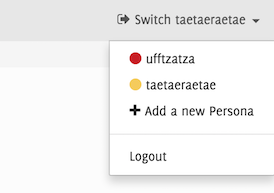
\includegraphics{img/switch.png}
\caption{The \emph{switch} menu lets users activate or create other
personas}
\end{figure}

On initial signup, new users create their first persona by giving it a
name and assigning a color to mark this persona's submissions. Following
completed signup, users can create more personas using the \emph{switch}
menu in the upper right corner of every screen. They can also choose to
create a new persona any time they are joining a movement. Therefore,
they can keep their membership in that movement separate from activities
in other parts of the site.

Other users can not tell whether any two personas are linked to the same
user account.

This functionality affords users of Rktik more freedom in managing their
online identity than comparable social platforms as described in
\hyperref[state-of-the-art]{State of the Art}. These freedoms may be
used to act out different social roles or to voice unpopular opinions
without fear of backlash against a user's offline identity. The notion
that there does not necessarily exist a 1:1 mapping between offline and
online identity is further established through the concepts of group
identity and agency.

\subsection{Personal vs.~Group
Identity}\label{personal-vs.group-identity}

Groups communicate their identity in online social networks through the
contents they publish and markers in the group's online representation
(group name, picture, color scheme). Rktik furthers this concept by
communicating not just a movement's identity but also its \emph{agency}.
The sense that a movement can think and act is established through 1)
terminology in the user interface that suggests a shared mind and 2)
features which let members use this shared mind to act collectively.

Language used in the context of movements implies that their members
have a shared mind: A movement's space for internal discussion and
exchange is called \emph{mindspace} and users place contents in
movements by \emph{creating thoughts} in the mindspace. This terminology
implies that members control a shared mental space, which they can use
to exchange thoughts. This notion is even stronger in private movements,
where only members can read thoughts in the mindspace.

A movement's agency is implied in the functionality of the movement
blog. Its contents are not dictated by a designated member of the
movement, but selected collectively by voting on thoughts in the
movement. The movement members make decisions collectively, which are
then attributed to the movement as a whole. Please see section
\hyperref[movement-agency]{Movement Agency} for possibilities for
further development of the concept of movement agency.

\hyperdef{}{movements}{\subsection{Movements}\label{movements}}

Movements allow groups of users with a shared interest to exchange their
thoughts about it. Any user may create new movements by specifying a
name and optional mission statement. A movement may also be created with
the \emph{private} option, which will hide contents of the movement
mindspace from non-members and only allow users with an invitation code
to join the movement as a member. These invitation codes may be created
by any movement member.

Users can access a movement by visiting its blog or mindspace, the
latter of which includes the movement's chat room. Members can post
thoughts to the movement mindspace by using the \emph{create thought}
interface or posting to the movement chat. Mindspace contents are sorted
by their hotness value (see \hyperref[hotness]{Distributing Attention:
Voting and Hotness}).

\hyperdef{}{promoting-content}{\subsubsection{Promoting
Content}\label{promoting-content}}

Movements automatically repost thoughts on their blog once they have
reached a certain number of votes. A progress bar, displayed alongside
each thought in the mindspace, indicates how many more votes are
required for promotion. This threshold value depends on the number of
group members. Please see section \hyperref[movement]{Movement} for
details on the implementation of the threshold function.

Movements are similar to Facebook Groups, Reddit's Subreddit feature and
Email newsgroups. All of them distinguish between private and public
groups as Rktik does; however, they do not provide group members with
the ability of democratically deciding to publish content publicly.

\hyperdef{}{private-movements}{\subsubsection{Private
Movements}\label{private-movements}}

When creating a new movement, a user may choose to make it
\emph{private}, which 1) hides the movement mindspace from non-members
and 2) only allows users with a valid invitation code to enter the
movement.

Invitation codes can be sent by movement members by either entering the
email addresses of invitees or by copying a URL with an embedded
invitation code and sending this to the invitee (e.g.~using a messenger
application).

The blog page of private movements indicates the movement founder so
that users interested in joining may contact this founder and ask for an
invitation.

\hyperdef{}{context}{\section{Context}\label{context}}

Every thought is linked to the context in which it was created. This can
either be the mindset in which a thought is submitted or another thought
in the case of replies. Reposts have both kinds of contexts as they are
created as replies on their original thought and simultaneously placed
directly in a specific mindset, effectively linking discussion in two
separate areas of Rktik.

\begin{figure}[htbp]
\centering
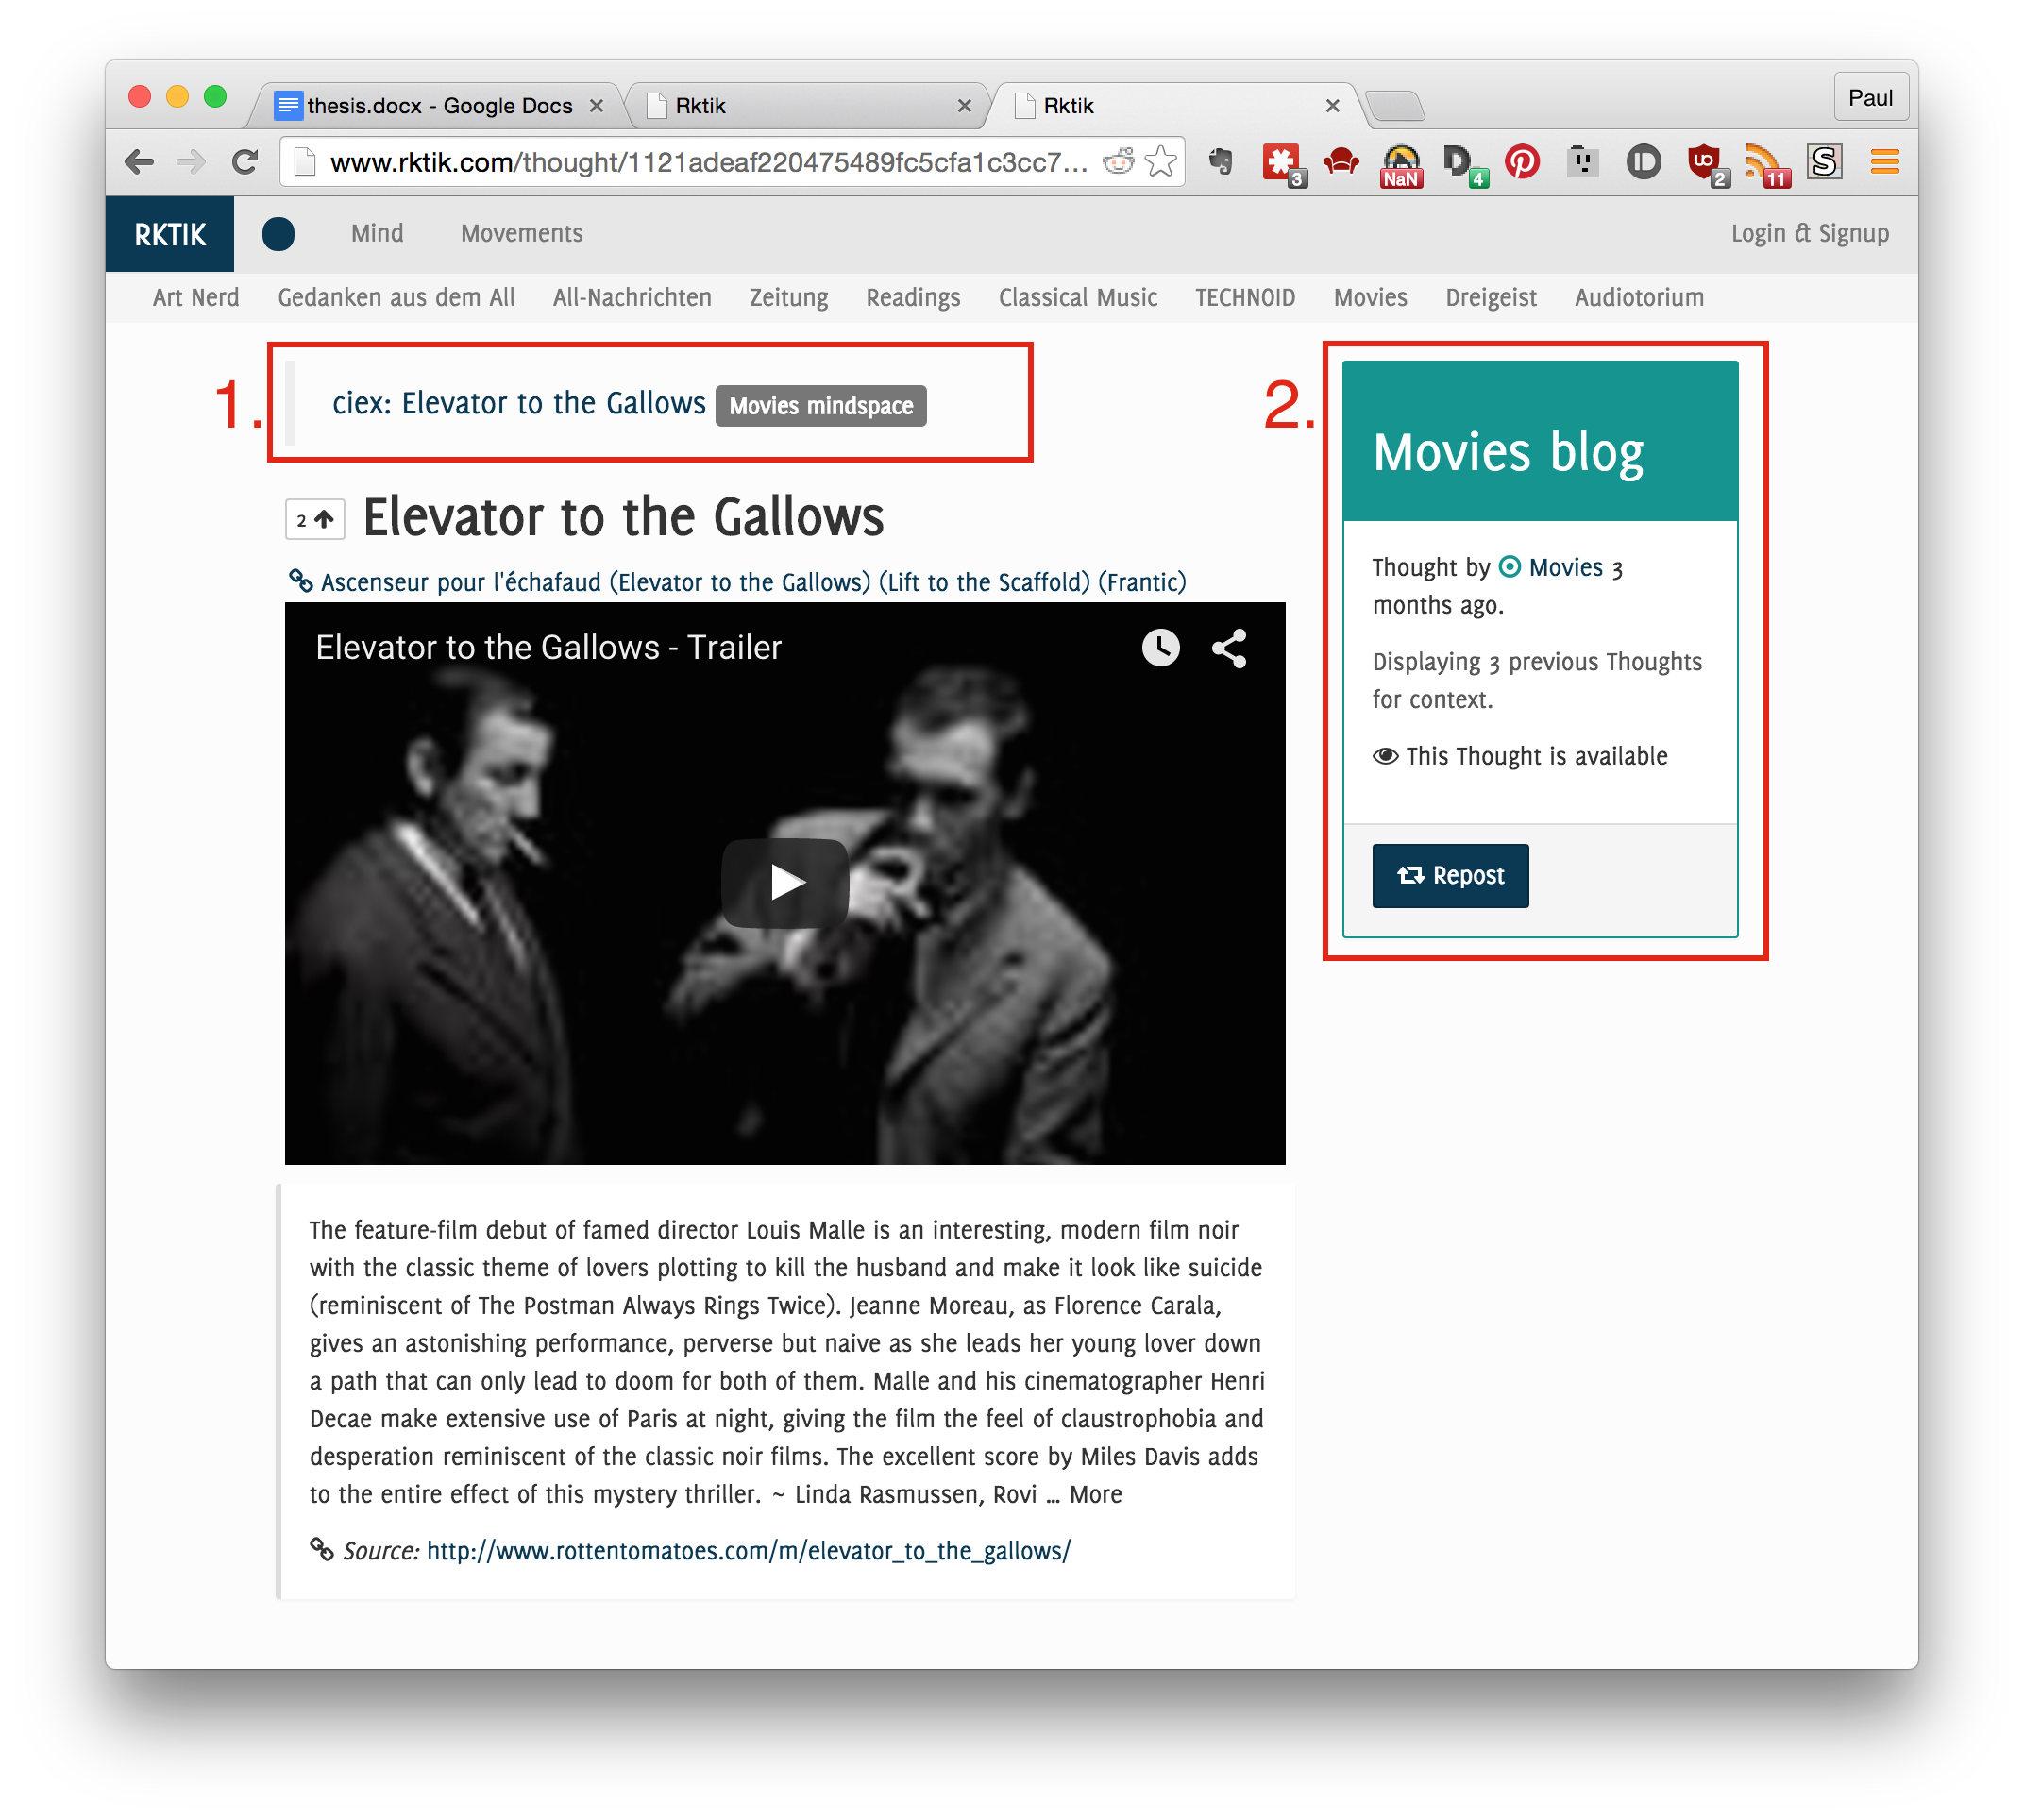
\includegraphics{img/context.png}
\caption{Reposts always have two contexts, marked red in this
screenshot: 1) The original thought, created in \emph{Movies mindspace},
to which this one is a reply and 2) \emph{Movies blog}, the mindspace in
which this repost was placed.}
\end{figure}

Mindsets are collections of thoughts, owned by identities. There are
three different kinds of mindsets for 1) internal thoughts of an
identity (mindspace), 2) its published thoughts (blog), and 3) private
conversation (dialogue). Each of them is rendered with a particular
layout and functionality.

This section will show how communication happens in the context of a
single thought, as well as in mindsets. Then, the differences between
the three kinds of mindsets are explained through their requirements,
tasks and conceptual design.

\subsection{Threaded Discussion}\label{threaded-discussion}

Every thought in Rktik has its own page which collects all information
related to the thought. This includes its text content and percepts as
well as the thought's context, metadata and reactions to it. Reactions
may be replies, reposts or automatic promotions (see
\hyperref[promoting-content]{Promoting Content}).

Displaying reactions to a thought in a flat listing can make it harder
for readers to follow the exchange as conversations regarding different
aspects of the original thought may be interweaved in the listing. Rktik
solves this problem by using a hierarchical display of reactions: Direct
replies are aligned to the left-hand side of the screen with subsequent
replies indented to the right. Further, every subsequent subtree of the
discussion is sorted by hotness.

\begin{figure}[htbp]
\centering
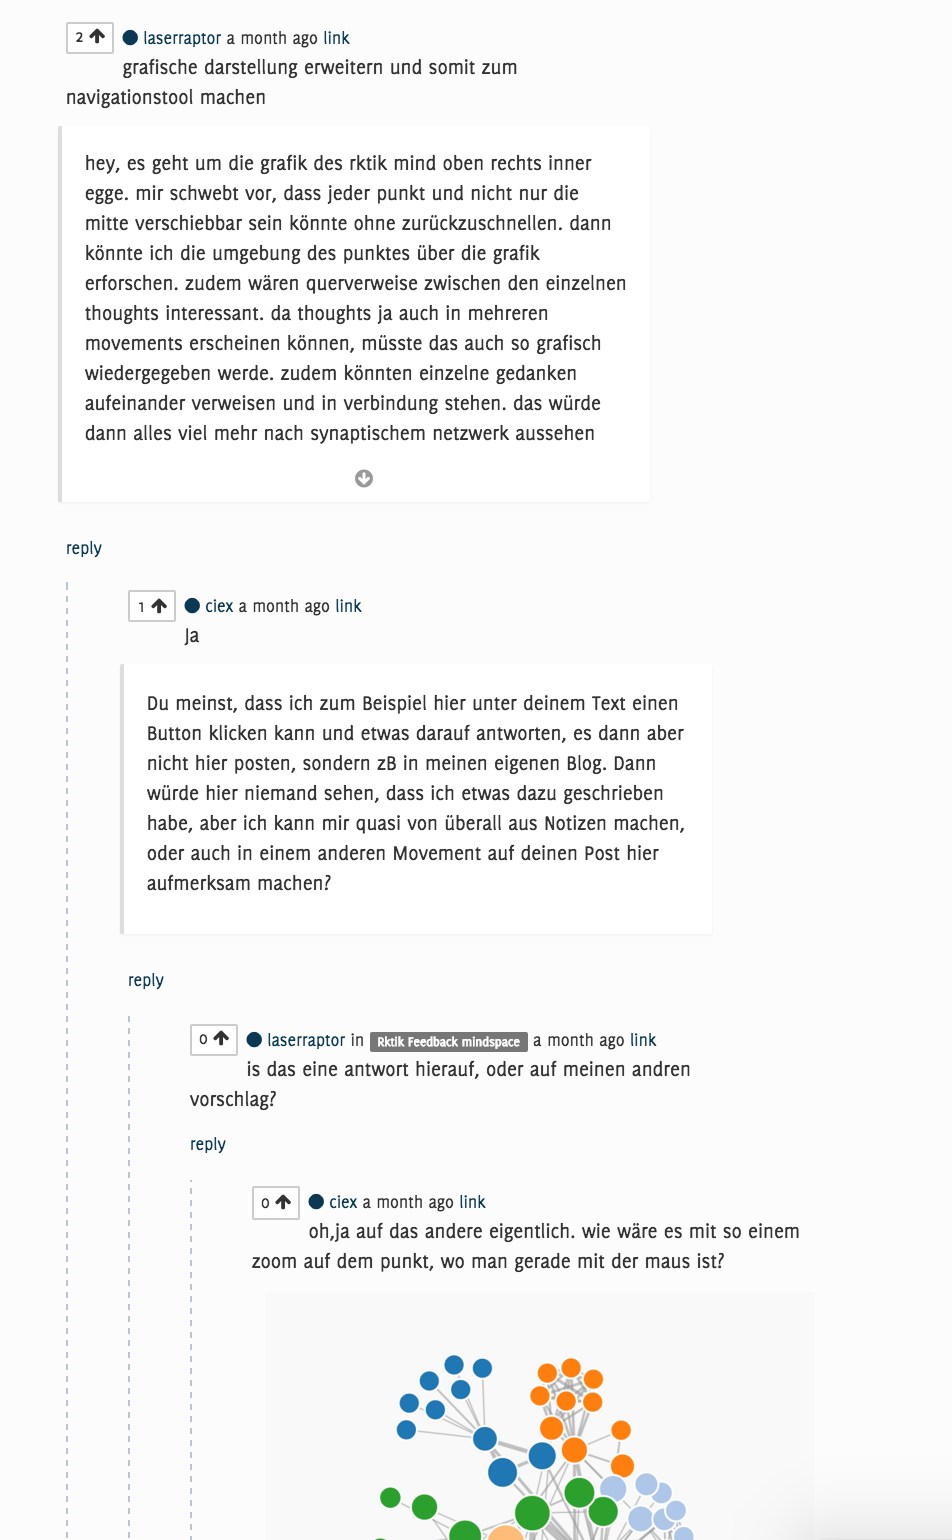
\includegraphics{img/comment_tree.png}
\caption{Comment tree with a depth of three replies}
\end{figure}

For performance reasons, the reaction tree depth is limited to three
levels. If a reaction is located in a mindset different from that of the
original thought, reactions happening in the other context are also
included up to a total depth of three levels.

If the original thought was created as a reply itself, the page also
contains its parent thoughts. The thought's author may define from 0-10
levels, how deep the reply-chain is recursed upwards for this purpose by
setting the context-depth setting on the left side of a thought's page.
Setting it to zero hides the thought's context from other users and
removes it from the discussion pages of these ancestors (TODO: reference
figure ``context.png'').

\subsection{Contextual Rights
Management}\label{contextual-rights-management}

Depending on context, a different set of identities is authorized to
create, edit and delete thoughts in a given mindset. See {[}Rights
Management{]} for detailed information about which users are authorized
for which actions.

\subsection{Mindspaces}\label{mindspaces}

Mindspaces are the first of three kinds of mindsets. They collect
internal thoughts of an identity as opposed to thoughts published on a
blog which is directed at a wider audience. Personas and movements are
both identities in Rktik and therefore have their own mindspace. The
differences between personal and collective mindspaces are described in
what follows.

\textbf{Persona Mindspace}

Every persona has access to their private mindspace in which only they
can read and write. This makes it a space for collecting thoughts before
deciding on whether or not, or in which context to publish them. The
mindspace of a persona is also referred to as the persona's
\emph{notebook} to make it easier for new users to understand how they
can use this feature.

Apart from creating thoughts directly in this mindset, users may also
use the \emph{repost} interface (see \hyperref[reposts]{Reposts}) to
copy thoughts from anywhere on the site into their notebook.

\textbf{Movement Mindspace}

\begin{figure}[htbp]
\centering
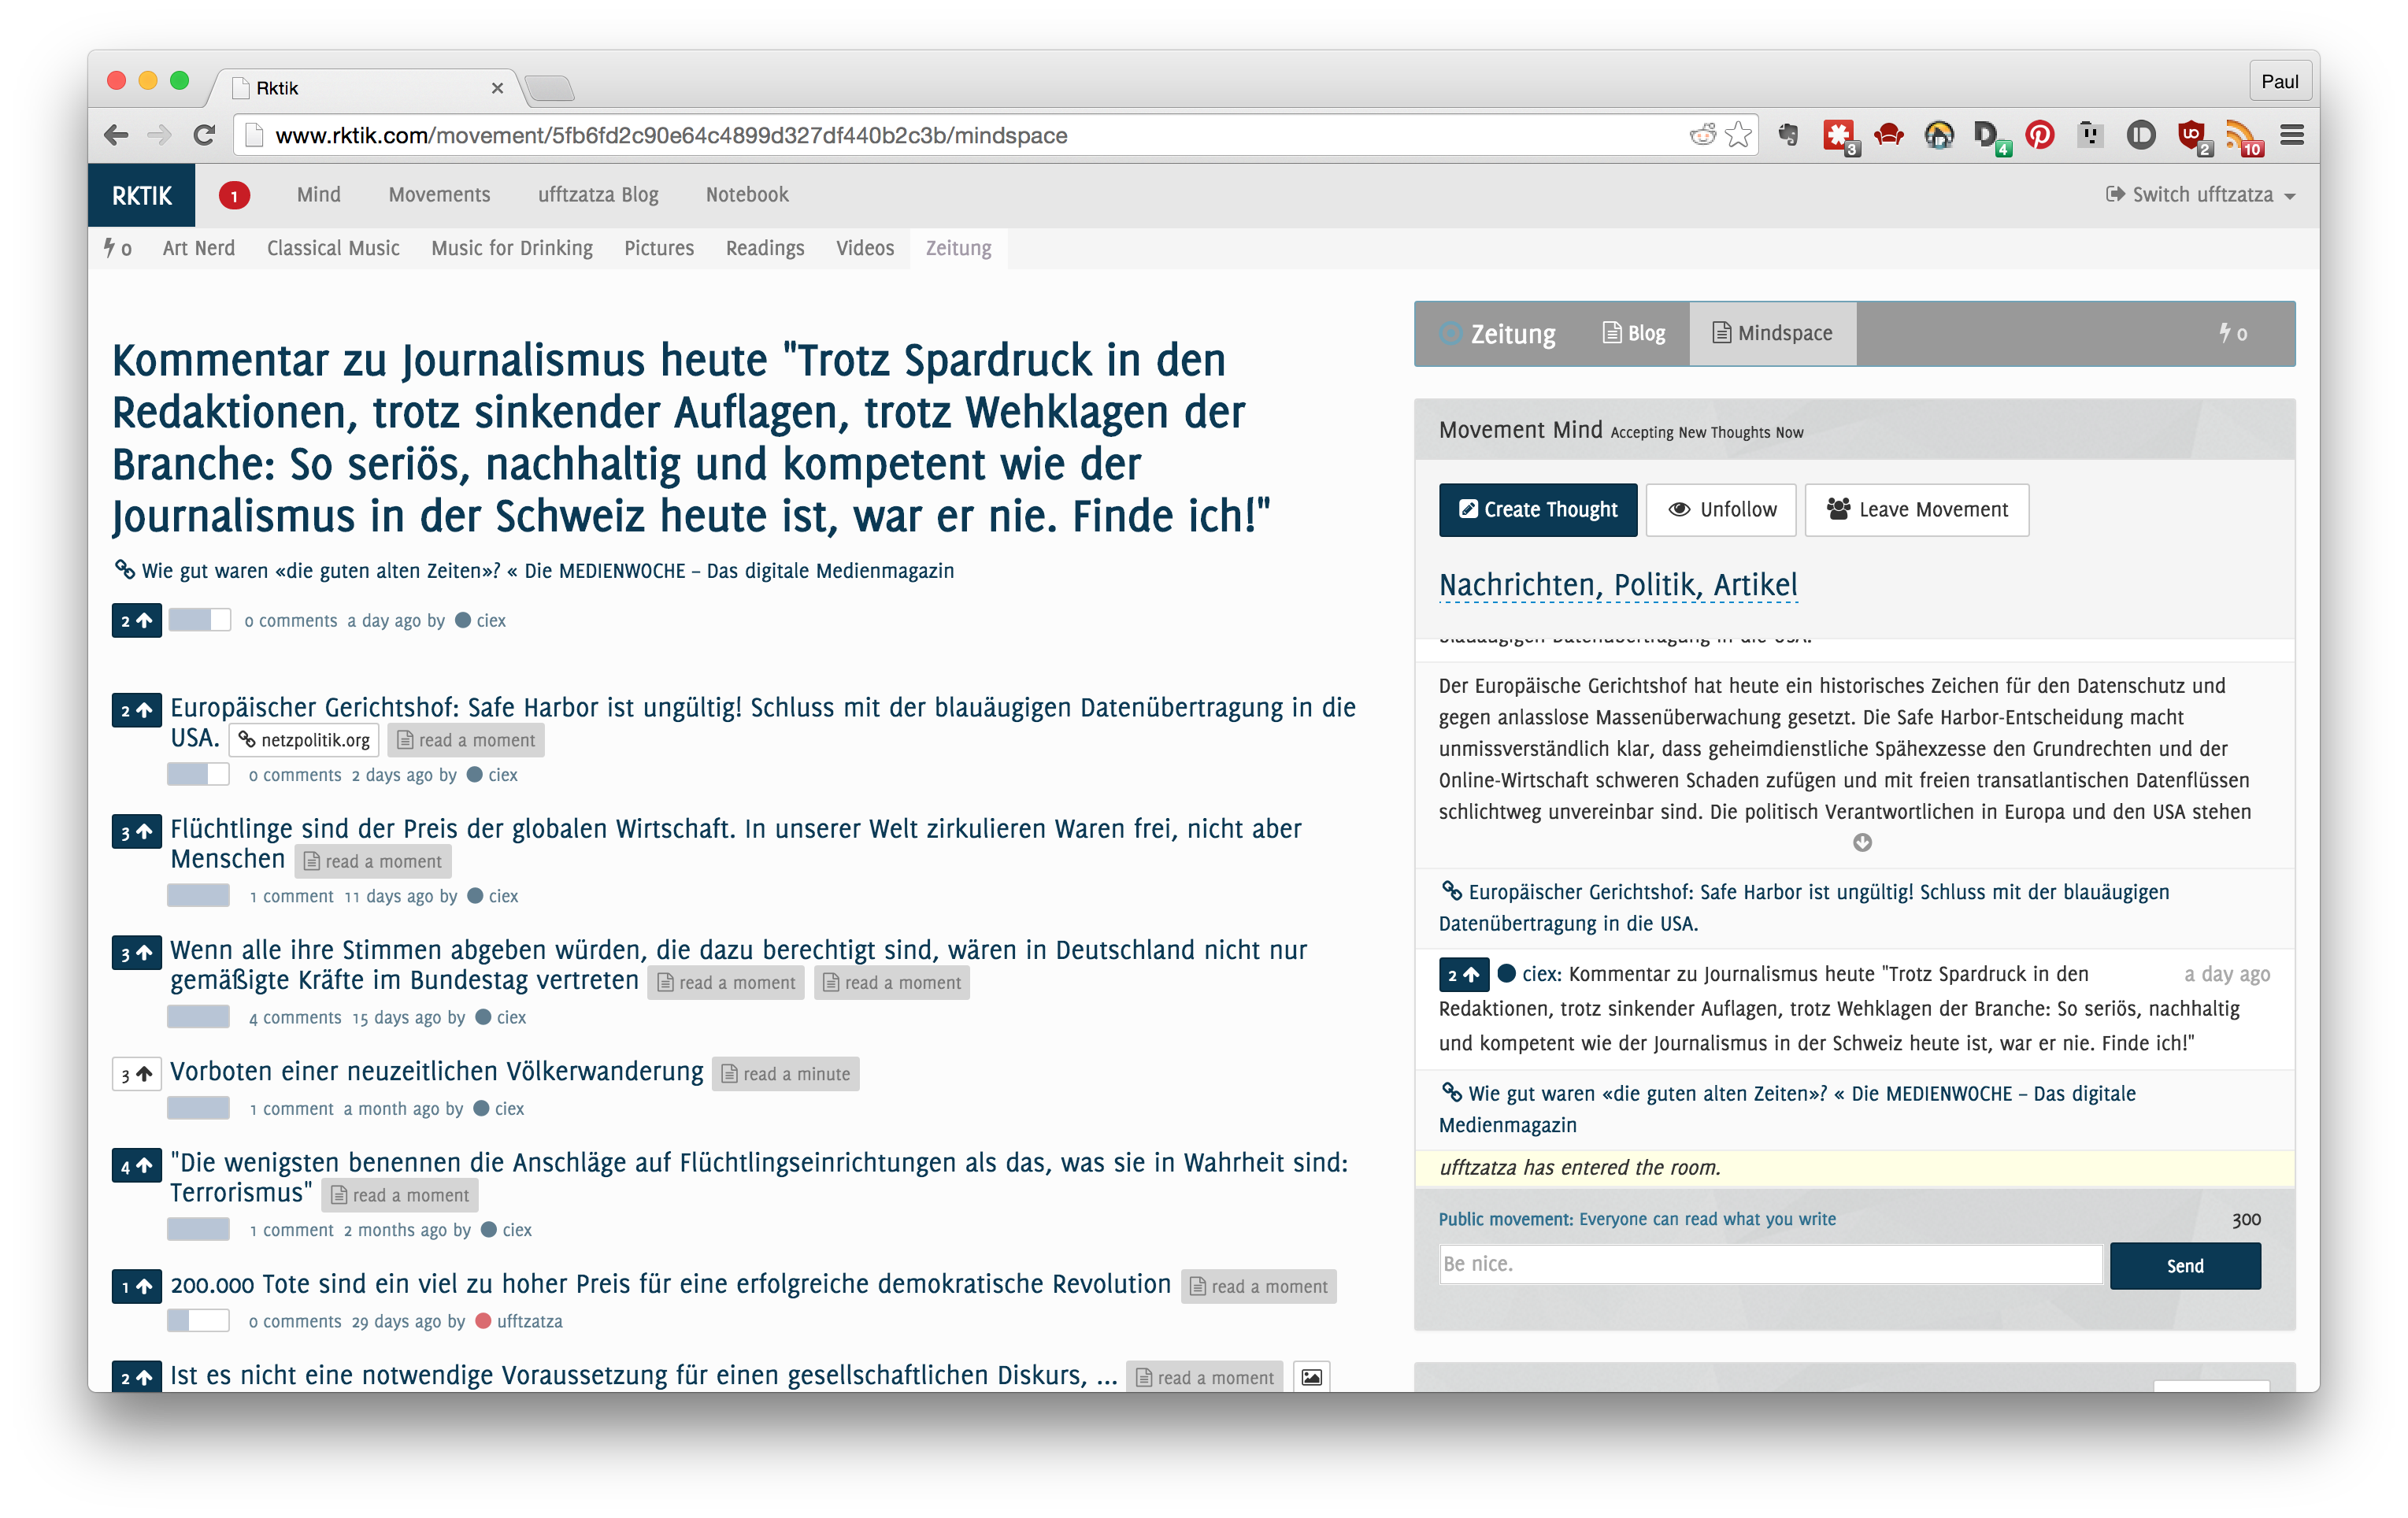
\includegraphics{img/mindspace.png}
\caption{Movement mindspace showing thoughts sorted by hotness on the
left and the movement chat on the right}
\end{figure}

The movement mindspace is the primary interface for movement members.
This space is facilitating discussion and exchange between movement
members and serving as a staging area for content that might be posted
to the movement's blog. The movement mindspace should therefore 1)
provide an overview of the most interesting content recently posted to
the mindspace and 2) provide members with a way to communicate directly
and immediately. To fulfill both of these requirements, the layout
displays thoughts both as a listing sorted by hotness as well as using a
chat widget.

While the chat is an automatically updating view of the most recent
thoughts, the listing changes more slowly. As the hotness ranking is
based on recency and number of votes, it is akin to a rolling toplist of
the currently most interesting thoughts. These thoughts can collect more
votes in the listing view until they reach the threshold for promotion
to the movement's blog (see \hyperref[promoting-content]{Promoting
Content}). A short blue bar displayed underneath each listing entry
indicates how many further votes are required for a promotion.

\hyperdef{}{chat}{\subsubsection{Chat}\label{chat}}

The chat should provide members with a sense of direct and immediate
participation in the movement. It provides an automatically updating,
chronological listing of all events related to the movement, including
all thoughts submitted to the movement mindspace and thumbnails of media
attachments.

This allows for a different mode of communication from the listing view
and threaded discussion. The immediate transmission of messages allows
the use of language with a conversational tone and creates the sense of
a more direct exchange between participants.

Replies to any thought in the movement mindspace are also displayed in
the chat. They come with an annotation that explicitly marks them as
replies and provides a hyperlink to their context. This allows movement
members watching the chat to directly start participating in these
discussions.

An inline form UI below the chat message listing allows users to send
thoughts to the mindspace/chat. Submitting the form clears the input
without reloading the page, so that the user can enter another message
immediately. Above the input, a notification text informs the user about
the privacy of messages entered, which is dependent on whether the
corresponding movement is private or not (see
\hyperref[private-movements]{Private Movements}).

\subsection{Blogs}\label{blogs}

Blogs are mindsets which allow identities to share their thoughts with a
wider audience and are sorted in reverse chronological order. Any
persona can follow any blog. Doing so places the blog's contents in the
pool of thoughts eligible for that user's personal frontpage.

Personas can directly post new thoughts to their personal blog, while
movement members can only indirectly place content in a movement's blog
through voting (see \hyperref[promoting-content]{Promoting Content}).

\subsection{Dialogue}\label{dialogue}

While mindspaces allow exchange \emph{between} many users, and blogs
allow broadcasting \emph{to} many users, the dialogue mindset models a
conversation between just two participants. As dialogues are also
implemented as a mindset, messages can be reposted freely between a
dialogue and any other context.

Apart from the different privacy setting, a dialogue provides the same
affordances as the chat module in a movement mindspace (see
\hyperref[chat]{Chat}).

\begin{longtable}[c]{@{}ll@{}}
\caption{Context in Rktik}\tabularnewline
\toprule
Context & Visible for\tabularnewline
\midrule
\endfirsthead
\toprule
Context & Visible for\tabularnewline
\midrule
\endhead
Blog & Everyone\tabularnewline
Mindspace (persona) & Only author\tabularnewline
Mindspace (private movement) & Members\tabularnewline
Mindspace (public movement) & Everyone\tabularnewline
Dialogue & Participants\tabularnewline
Reply & Determined by the original thought\tabularnewline
\bottomrule
\end{longtable}

\chapter{Implementation and
Operation}\label{implementation-and-operation}

\section{Overview}\label{overview-1}

This chapter gives technical information about the implementation and
operation of the Rktik service.

The chapter starts with a section on the shared data model
\emph{Nucleus}. Following is a section on the \emph{Glia} web server.
Finally comes a description of performance improvements and the details
of deployment and operation of Rktik in a hosted environment .

\section{Shared Data Model: Nucleus}\label{shared-data-model-nucleus}

The Nucleus library uses the SQLAlchemy ORM\footnote{\href{https://pypi.python.org/pypi/SQLAlchemy/0.9.2}{SQLAlchemy
  0.9.2}} to provide data persistency and defines methods for
context-independent data processing. It is implemented as a Python
package which can be imported from the main application \emph{Glia}. The
Nucleus package also provides a direct database connection that can be
used from Glia to bypass the ORM layer, as well as a connection to the
in-memory cache \emph{memcache}. A signalling namespace provides event
hooks which are used to automate post-processing and other tasks in
reaction to model changes.

As Rktik was planned as a semi-decentralized service\footnote{Semi-decentral
  in this case means that users can chose between 1) a client
  application for rendering and processing data which uses a web server
  for the transfer of (encrypted) data and 2) solely using Rktik on its
  website without installing an application on their computers.}, the
object relational manager was decoupled from the rest of the application
from the beginning to allow for the easy implementation of client and
server applications using this codebase.

The following subsections will describe the components of the Nucleus
package, namely the \emph{Serializable} module and ORM models. The last
subsection will give general information about database development
using the SQLAlchemy ORM.

\hyperdef{}{serializable}{\subsection{Serializable}\label{serializable}}

The \emph{Serializable} module primarily provides serialization
capabilities to ORM models that inherit from it. This functionality is
not in the scope of this thesis, but part of the planned P2P extension
(see \hyperref[external-clients]{External Clients}). As the module is
also required for rights management, I have left it in the codebase
submitted along with this document, and will describe the relevant
functionality here.

Serializable instances provide a method \emph{authorize}, which
validates that a given user may execute a specific action on the
instance. An action may be creating, updating or deleting specific data
stored in the instance, such as a persona's username or a thought's
title. Each model that inherits from \texttt{Serializable} can define
its own handling of user rights by overriding this method. Please see
{[}Rights Management{]} for detailed information on which users are
allowed to make changes to which objects.

\hyperdef{}{nucleus-models}{\subsection{Nucleus
Models}\label{nucleus-models}}

The module \texttt{nucleus.models} contains definitions for all ORM
models. Each model is represented by a class definition. See {[}API
specification{]} for technical details such as the attributes and
methods provided by each model. This section gives an overview for each
model's properties and responsibilities with respect to the
functionality described in the \emph{conceptual} chapter.

\begin{figure}[htbp]
\centering
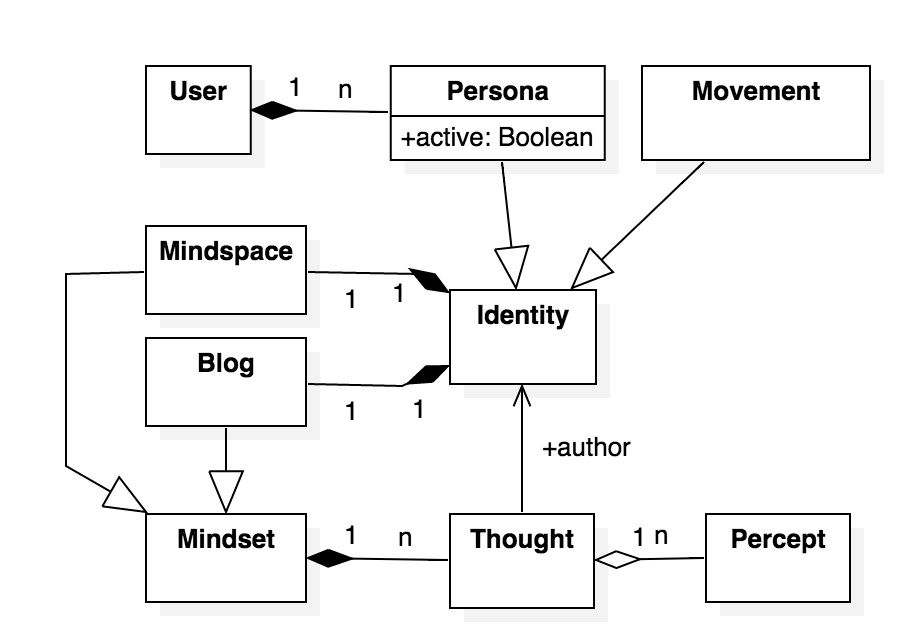
\includegraphics{img/terminology.png}
\caption{Class diagram of important classes and relations in Rktik as
described in \hyperref[nucleus-models]{Nucleus Models}. Most attributes
and operations have been omitted for simplicity.}
\end{figure}

\subsubsection{User}\label{user}

The \texttt{User} model represents a registered user of the site. It has
relations to all personas of this user and stores basic metadata such as
the user ID, account creation data, email and password hash. The
\texttt{User} class is also used in verifying user's email addresses and
storing the validation state related to the user.

\subsubsection{Identity}\label{identity-1}

The \texttt{Identity} class is a superclass for \texttt{Persona} and
\texttt{Movement} as these two share many attributes and methods related
to them being identities.

Apart from basic information such as username, user color, creation and
modification timestamps, the \texttt{Identity} model has relations to
the blog and mindspace associated with each instance.

\subsubsection{Persona}\label{persona}

The \texttt{Persona} class represents personal identities taken by users
of the site. Each \texttt{User} instance may be connected to many
\texttt{Persona} instances.

The \texttt{Persona} model provides methods for toggling instances'
memberships in movements and following and unfollowing blogs. It also
provides a number of cached methods that serve as shortcuts to
information related to the Persona which is computationally expensive to
collect (see \hyperref[improving-performance]{Improving Performance}).

\hyperdef{}{movement}{\subsubsection{Movement}\label{movement}}

Just as the \texttt{Persona} model, \texttt{Movement} instances inherit
from the \texttt{Identity} model and thereby provide all its attributes
and methods. They also store the movement's mission, whether the
movement is private and relations to the movement's admin (founder) and
to movement members.

When votes are cast on thoughts in the movement mindspace, the
movement's \texttt{promotion\_check} method is called. This method
reposts the thought to the movement blog, if the number of votes passes
a threshold. Given the number of members (c) the threshold value (t) is
defined as:

\begin{verbatim}
t = round(c / 100 + 0.8 / c + log(c, 1.65)) if c > 0 else 1
\end{verbatim}

This formula ensures that for a small movement a low number of votes is
required, thus creating lots of content on the blog. At the same time
larger movements need more votes relative to their user count, so that
only the best content will be posted to the blog.

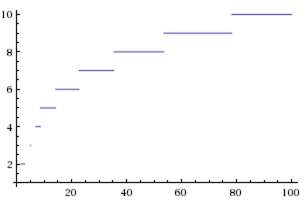
\includegraphics{img/threshold_1.png}\\
 Plot of threshold function for c = 1 to 100.

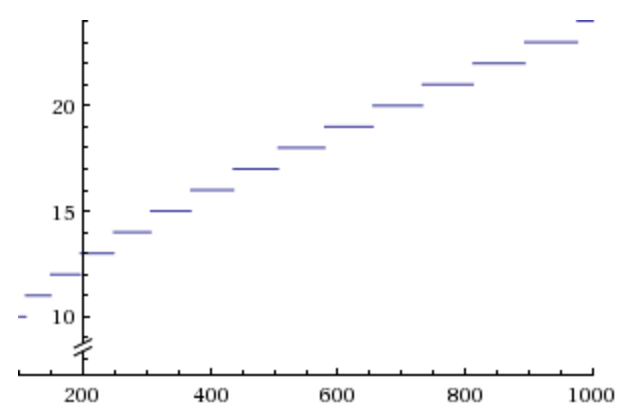
\includegraphics{img/threshold_2.png}\\
 Plot of threshold function for c = 100 to 1000.

\textbf{Movement Member Association}

The members relation is implemented using the
\href{http://docs.sqlalchemy.org/en/rel_1_0/orm/basic_relationships.html\#association-object}{association
object pattern} to store additional metadata about the membership. This
pattern uses an additional table to represent relations between two
entity classes. This table can be used to record additional information
about the relation:

\begin{itemize}
\tightlist
\item
  \texttt{active} (Boolean): Inactive memberships are used to represent
  former members and for invitations. The latter are created as inactive
  memberships with no associated persona.
\item
  \texttt{created}, \texttt{modified}: Timestamps for creation and last
  modification of the membership.
\item
  \texttt{role}: The member's role in the movement (currently one of
  ``member'' and ``admin'').
\item
  \texttt{last\_seen}: Time when the persona was last present in the
  movement chat
\end{itemize}

\subsubsection{Mindset}\label{mindset}

This model represents a \emph{set of thoughts} with an author and is a
superclass of \texttt{Mindspace}, \texttt{Blog} and \texttt{Dialogue}.

\begin{itemize}
\tightlist
\item
  \textbf{Mindspace} models internal thoughts of an identity
\item
  \textbf{Blog} models a blog publication
\item
  \textbf{Dialogue} models a conversation between two identities. The
  dialogue model has an additional relation to personas representing the
  ``other'' of a conversation. This means that retrieving the dialogue
  between two given personas is not a simple lookup, as the
  \texttt{author} and \texttt{other} attribute can be filled
  interchangeably. Therefore, a \texttt{get\_chat} classmethod is
  provided that probes the two lookup possibilities in succession and
  returns a new dialogue instance if both are unsuccessful.
\end{itemize}

\subsubsection{Thought}\label{thought}

The \texttt{Thought} model represents content submissions by users of
the site. Each instance stores the title text and metadata of the
thought. All other media related to the thought is contained in
\texttt{Percept} objects. Thoughts also store the context they were
posted in, which may either be a parent thought for replies or a mindset
for top-level thoughts.

The thought class is able to generate instances of itself directly from
text input received via the UI through a classmethod. This process
includes detecting embedded URLs and validating whether they refer to a
\emph{valid} HTTP resource, creating \texttt{Percept} objects for any
text, link or linked picture attachments, relaying notifications
triggered by the creation of new thought and percept instances and
invalidating caches touched by the new thought.

Thoughts also have a relation to their votes and helper methods for
accessing information about these votes (has a specific user voted,
total amount of votes, hotness value).

\subsubsection{Upvote}\label{upvote}

The \texttt{Upvote} model inherits from \texttt{Thought}. Its instances
represent votes cast by personas on other thoughts. This relation is
represented by the upvote instance referring to the voted thought as its
parent.

\subsubsection{Percept}\label{percept}

The \texttt{Percept} model represents attachments on thoughts. The
\texttt{Percept} class is thereby used as an abstract class with
following subclasses:

\begin{itemize}
\tightlist
\item
  \texttt{LinkPercept}, \texttt{LinkedPicturePercept}: Store a URL link,
  which is rendered inline in case of the \texttt{LinkedPicturePercept}
\item
  \texttt{TextPercept}: Stores the attached text
\item
  \texttt{MentionPercept}: Stores a relation to the linked user and the
  text used to refer to them (these might be different if the mentioned
  persona changes their username after being mentioned)
\item
  \texttt{TagPercept}: Store a relation to an instance of the
  \texttt{Tag} model (see \hyperref[tag]{Tag}).
\end{itemize}

Percepts are linked to a thought with the association object pattern.
The \texttt{PerceptAssociation} class stores the author who created the
association in addition to its thought and percept. The association's
author is usually identical with the thought author, but movement admins
also have the rights to edit thoughts submitted to their movement's
mindspace.

\hyperdef{}{tag}{\subsubsection{Tag}\label{tag}}

The \texttt{Tag} model represents labels attached to thoughts. Tags can
be created by adding the hash character `\#' as a prefix to any word in
the thought title or text. Tagged thoughts do not have a direct relation
with a tag instance but use the \texttt{TagPercept} model as an
association object. This way, tags can be renamed globally without
modifying all thoughts that have this tag.

\hyperdef{}{notification}{\subsubsection{Notification}\label{notification}}

Notifications represent direct messages to the user, generated
automatically when certain events require the user's attention. The
\texttt{Notification} base class stores metadata such as the
notification text, URL, unread status and recipient. Subclasses are used
to represent specific kinds of notifications:

\begin{itemize}
\tightlist
\item
  \texttt{MentionNotification}: Sent to a persona when a mention
  referring them is posted
\item
  \texttt{ReplyNotification}: Sent to a persona when they receive a
  reply on one of their Thoughts.
\item
  \texttt{DialogueNotification}: Sent for new messages in a private
  conversation between two Personas.
\item
  \texttt{FollowerNotification}: Sent to a persona when their blog gains
  a new follower.
\end{itemize}

\subsection{Modeling Data with
SQLAlchemy}\label{modeling-data-with-sqlalchemy}

SQLAlchemy allows the implicit specification of database schemas through
defining the Python classes that the database ought to model. It maps
user-defined Python classes to database tables and instances of these
classes to rows in the tables. Changes to instances are transparently
synchronized with database contents and queries for retrieving data can
be formulated in an object oriented expression language. This has the
advantages that 1) developers can start modifying the database schema
without having to learn a query language specific to the used database,
2) the connected database backend can be changed with minimal
modifications to the model specifications and 3) all code related to the
ORM models resides in one place, thereby limiting code fragmentation.

While SQLAlchemy makes the creation of a database easy in the beginning
of a project, it can later lead to performance problems. Reducing the
complexity of database access is appropriate for straightforward use
cases but can lead to inefficiencies in more complex scenarios. As
SQLAlchemy does not necessarily translate a given command into the most
effective query many advanced queries can be optimized with some
knowledge of how the underlying database is used. The library provides
an extensive suite of tools for implementing these optimizations.

When model definitions are changed while the database is already used in
production, it is not enough to recreate the database using the new
schema, as old data may have to be migrated. Rktik uses the Alembic
library\footnote{\href{https://pypi.python.org/pypi/alembic/0.7.5.post2}{Alembic
  0.7.5.post.2}} to record schema changes and migrate the database
layout. Schema migrations are automatically executed on the server by
the deployment script (see \hyperref[hosting-and-deployment]{Hosting and
Deployment}).

In cases where not only the database schema, but also its contents have
to be modified, migration scripts have to be manually written in
accordances with the changes. These are stored in the
\texttt{glia/migrations\_extra} directory for one-time execution on the
server.

\section{Web Server: Glia}\label{web-server-glia}

The \emph{Glia} web server is a Python package based on the Flask web
framework, and responsible for:

\begin{itemize}
\tightlist
\item
  collecting and computing contents of the user interface,
\item
  serving asynchronous UI updates,
\item
  validating, storing and modifying information entered by the user,
\item
  automatically performing maintenance operations, and
\item
  scheduling email delivery.
\end{itemize}

Glia consists of the following components:

\begin{itemize}
\tightlist
\item
  \emph{Views} are functions mapped to URL patterns and compute their
  contents when accessed by a user
\item
  \emph{Websocket events} are special views used for asynchronous
  communication with a web browser
\item
  \emph{Forms} validate restraints on structured user input
\item
  \emph{HTML Templates} are used to map data into a graphical layout to
  be rendered by a browser
\item
  \emph{Configuration files}
\item
  \emph{Database migration scripts}
\item
  \emph{Static files} (Images, frontend Javascript resources, etc)
\end{itemize}

\textbf{Session Management}

Session management is responsible for storing information about which
user is logged in on which browsers. Rktik uses the Flask-Login
extension\footnote{\href{https://pypi.python.org/pypi/Flask-Login/0.2.11}{Flask-Login
  0.2.11}} to provide most of this functionality.

Users can login using their email and password, which will let
Flask-Login store a cookie in their browser recording the logged-in
state.

\subsection{Web View and URL Routing}\label{web-view-and-url-routing}

Views are functions that return HTML content and are mapped by a route
to a URL scheme, which can be accessed by a user through a web browser.

The following section lists a description of all views available in
Glia. Some of these are \emph{redirect views}, which do not return a web
page to the browser but redirect it to a different URL.

\begin{itemize}
\tightlist
\item
  \textbf{index} Frontpage at (\url{http://rktik.com/})
\end{itemize}

\emph{Personas}

\begin{itemize}
\tightlist
\item
  \textbf{create\_persona} Form for adding a new persona
\item
  \textbf{notebook} Private area for storing notes and reposting
  thoughts for oneself
\item
  \textbf{notifications} Listing of notifications for active persona and
  email preferences for logged in user account
\item
  \textbf{persona} Basic information about a single persona and listing
  of all movements they are a member of. This view includes a chat
  widget for private conversations with other users.
\item
  \textbf{persona\_blog} Personal blog of a persona
\end{itemize}

\emph{Thoughts}

\begin{itemize}
\tightlist
\item
  \textbf{create\_thought} Dedicated page for creating new thoughts. In
  contrast to the inline thought creator this view also allows entering
  long text attachments.
\item
  \textbf{edit\_thought} Similar interface to the \emph{create\_thought}
  view that allows removing and editing attachments and the thought's
  title.
\item
  \textbf{delete\_thought} Confirmation dialog for removing thoughts.
\item
  \textbf{thought} View for a single thought that includes its context,
  attachments, comments and the thought's metadata.
\end{itemize}

\emph{Movements}

\begin{itemize}
\tightlist
\item
  \textbf{movement} Redirect view that sends members to a movement's
  mindspace and non-members to the movement blog.
\item
  \textbf{movement\_blog} Main listing for a movement's blog that
  presents a reverse chronological, paginated view of thoughts in the
  blog. Also allows following the movement and becoming a member.
\item
  \textbf{movement\_mindspace} View for movement mindspace contents as
  well as movement chat and basic movement metadata.
\item
  \textbf{invite\_members} Form for obtaining invitation links for a
  movement and sending email invitations.
\item
  \textbf{movement\_list} List all movements registered on Rktik
\end{itemize}

\emph{User account related}

\begin{itemize}
\tightlist
\item
  \textbf{activate\_persona} Redirect view that activates a different
  persona registered to the logged in user account
\item
  \textbf{signup} Form for creating a new user account
\item
  \textbf{signup\_validation} Redirect view for validating a user's
  email address
\item
  \textbf{login} Login form for user accounts
\item
  \textbf{logout} Redirect view that logs out the current user account
\end{itemize}

\emph{Helpers}

\begin{itemize}
\tightlist
\item
  \textbf{help} Access help pages stored in
  \emph{templates/help\_*.html} files
\item
  \textbf{tag} Listing of thoughts marked with a specific hashtag
\end{itemize}

\emph{Before request}

These special views have the \texttt{before\_request} decorator, which
causes them to be executed every time a user visits a page.

\begin{itemize}
\tightlist
\item
  \textbf{account\_notifications} Inserts a notification into the page
  if the logged in user has not validated their email address
\item
  \textbf{mark\_notifications\_read} Marks all notifications as
  \emph{read} which have a URL equal to the current page
\end{itemize}

\hyperdef{}{html-templates}{\subsection{HTML
Templates}\label{html-templates}}

Templates allow separation of content and layout in the application
backend and thereby lead to more readable code. They consist of layout
definitions written in HTML and additional markup that defines where
content needs to be inserted. View functions compute all information
neccessary for a given web page and then pass this information as
parameters to a template. Rktik uses the Jinja2 template
engine\footnote{\href{https://pypi.python.org/pypi/Jinja2/2.8}{Jinja2
  2.8}} included with Flask for this purpose.

Jinja2 provides almost all required functionality with missing features
made available through extensions. Rktik uses the \emph{humanize}
library\footnote{\href{https://pypi.python.org/pypi/humanize/0.5}{Humanize
  0.5}} for converting date and time data into a human readable
format.\footnote{As an example, instead of displaying
  \texttt{2015-10-01T15:42:23.254966+00:00} as a thought's creation
  time, the relative form \emph{two hours ago} is used} Additionally, a
number of custom filters are used in templates:

\begin{itemize}
\item
  Rktik stores all date and time information in the GMT timezone. This
  allows handling time information in the backend without considering
  time zones. A custom filter is used to convert these to European
  central time in the template.
\item
  The \emph{mentions} filter uses information from mention percepts (see
  \hyperref[nucleus-models]{Nucleus Models}) to replace occurrences of
  the pattern \texttt{@persona\_name} with a link to the respective
  persona's page
\item
  The \emph{gallery\_col\_width} filter is used to adapt the size of
  image attachments to their number. The largest format is used when
  only one image is attached. A successively smaller image size is used
  up to four image attachments.

  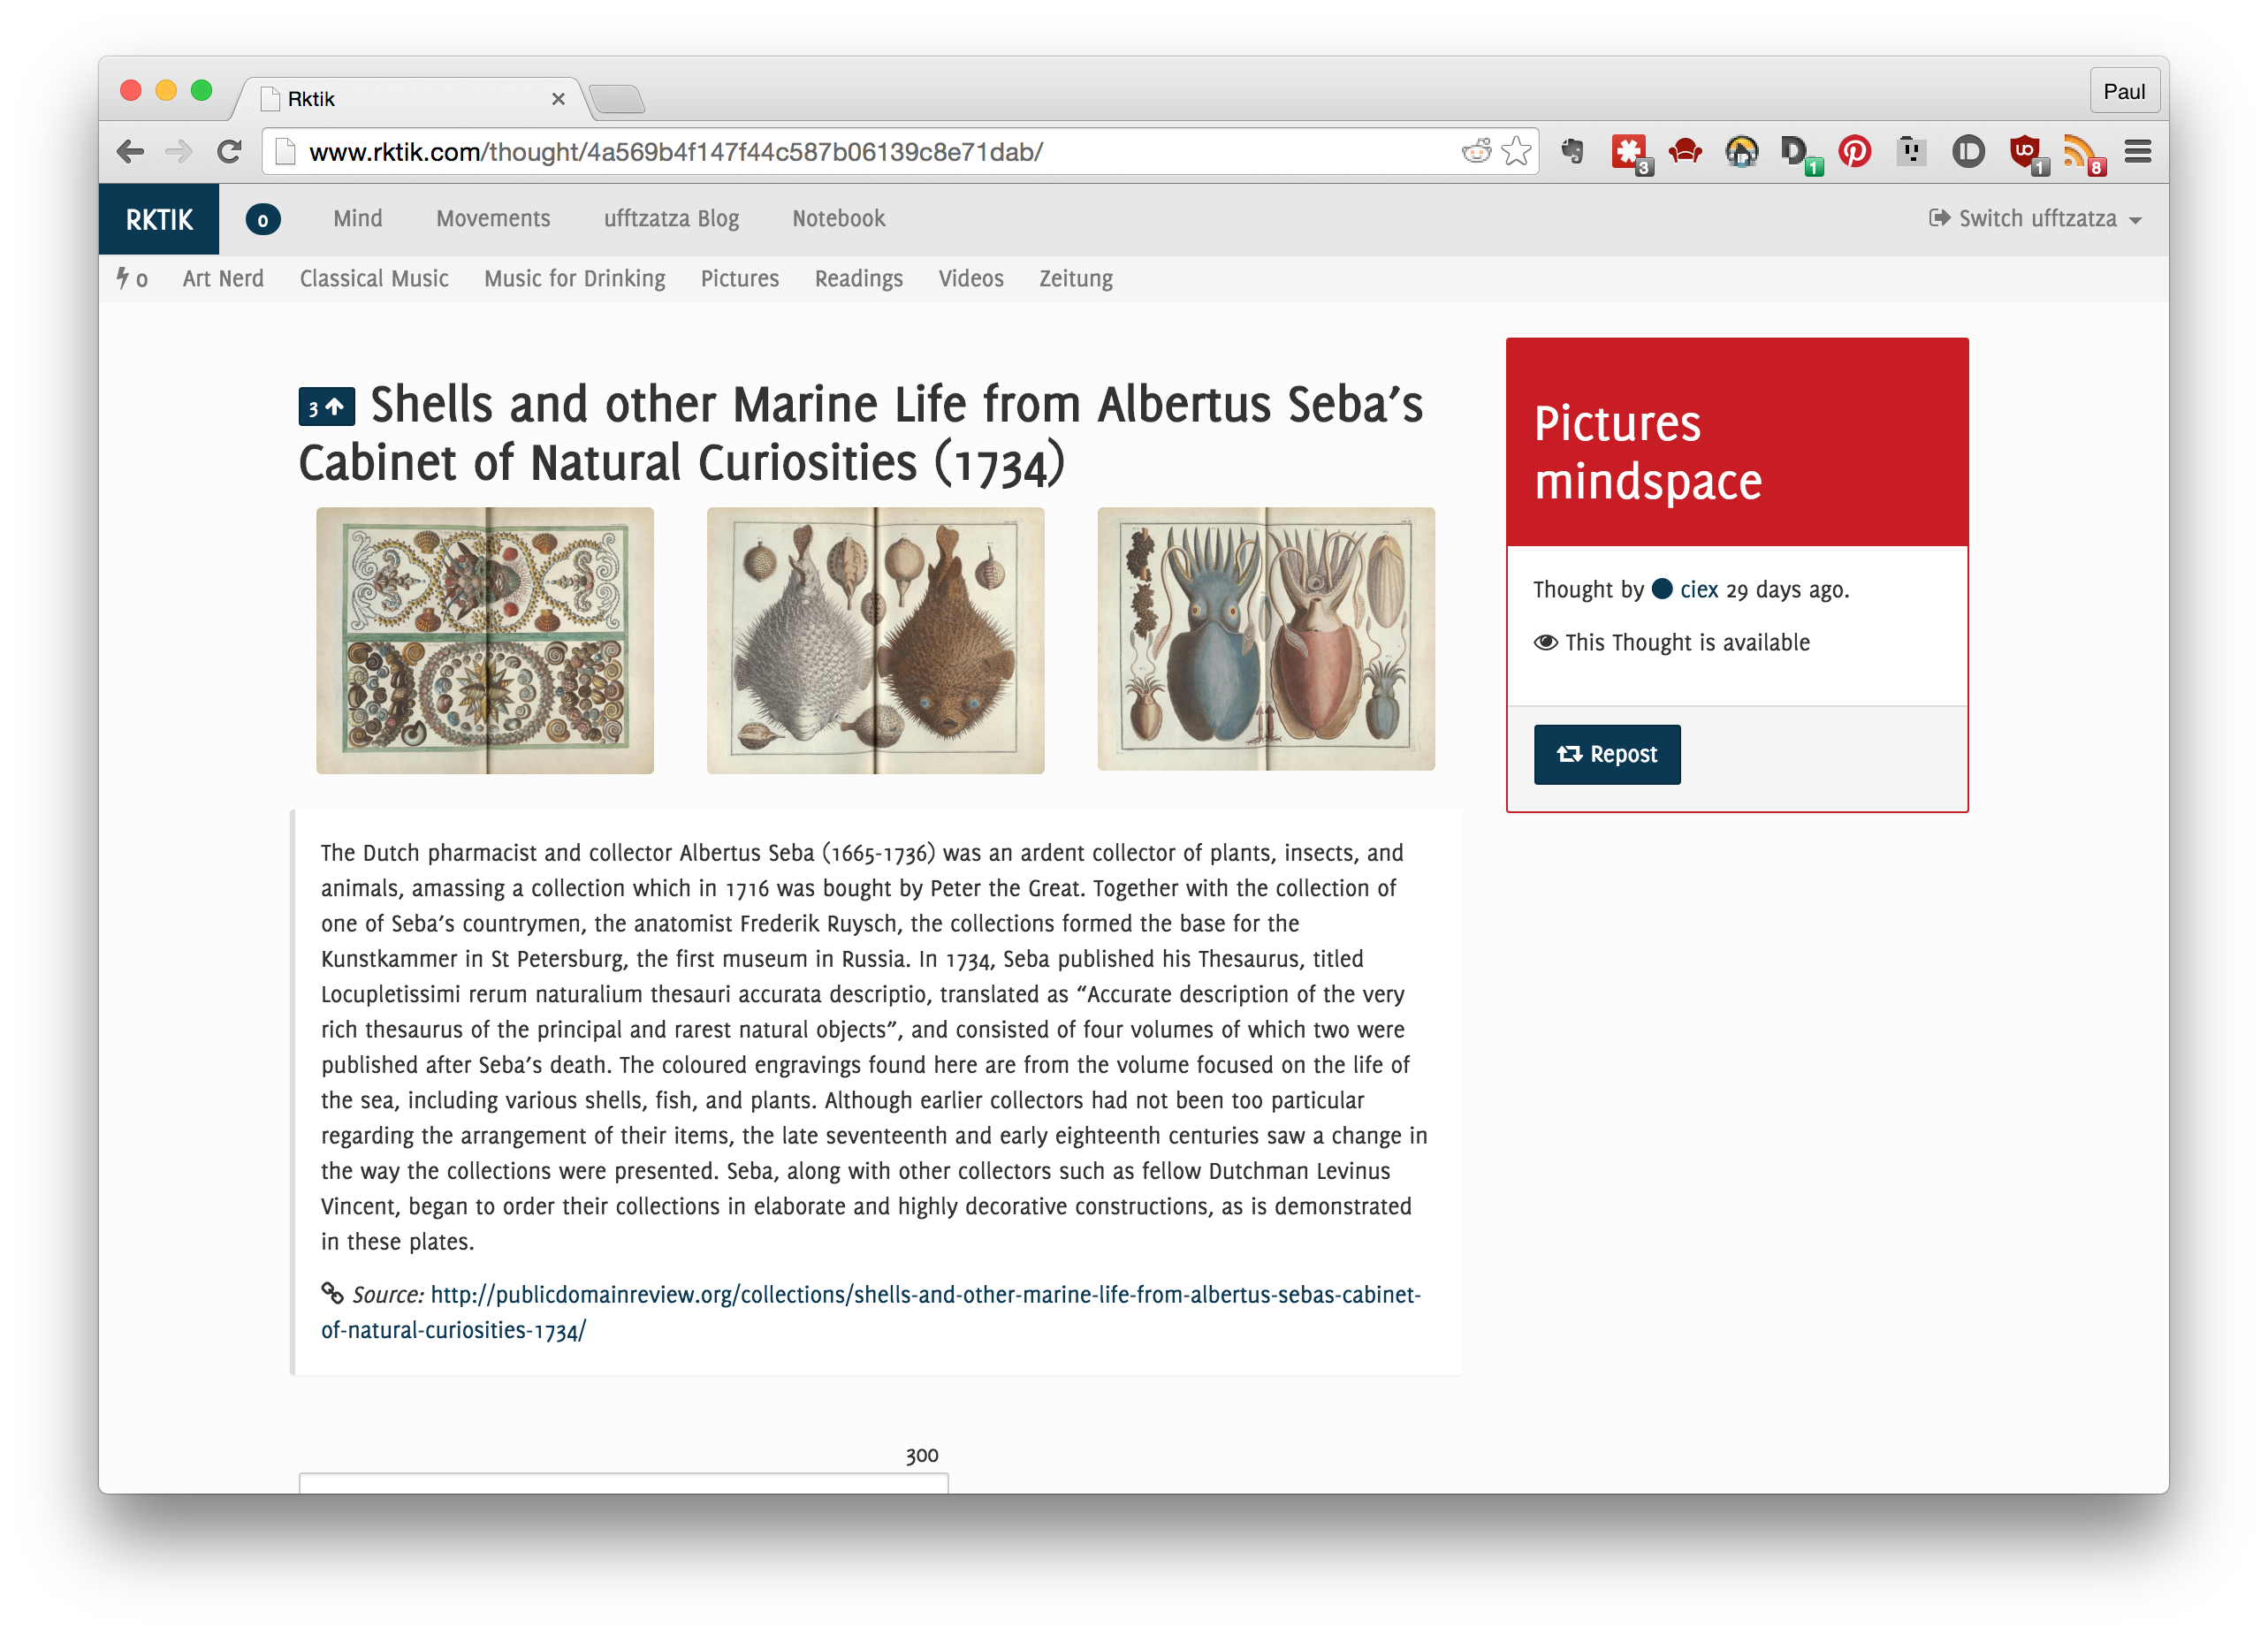
\includegraphics{img/col_width.png}
\item
  The \emph{sort\_hot} filter can be used to apply the hot ranking to
  lists of thoughts
\item
  The \emph{authorize} filter replaces thought contents with a
  placeholder if the thought is not visible to the active persona (see
  \hyperref[serializable]{Serializable}).
\end{itemize}

\subsection{Asynchronous UI}\label{asynchronous-ui}

Most of the content of Rktik is compiled on the server and then sent as
a complete web page to the user's browser. When an interaction requires
only part of the screen contents to be changed, site responsiveness is
increased by using asynchronous communication with the server. This
functionality is implemented using the \emph{jQuery} Javascript library
(\href{https://jquery.com/}{jQuery website}) for one-off asynchronous
calls and the \emph{websockets} browser technology for continuous
streams of information.

The websockets technology provides a socket between the browser and the
Glia server which is used for relaying information during the time in
which the browser window stays open. All thoughts created in a movement
mindspace including chat messages as well as all votes on these
thoughts, are received and immediately relayed by the server to all
browser windows that show part of the movement. Messages received on the
client side are inserted into the chat widget. If the browser window
shows an individual thought's page, new comments are inserted at the
appropriate place in the hierarchical comments view.

The same channel is used for sending reposts and receiving desktop
notifications (see \hyperref[notifications-1]{Notifications}). Server
side handlers for websockets are located in the \texttt{glia.web.events}
module, while client side handlers are located in the static file
\texttt{glia/static/js/main.js}.

Other asynchronous calls are handled using jQuery based javascript
functions. This includes:

\begin{itemize}
\tightlist
\item
  Loading more chat contents.\footnote{The chat window initially loads
    the most recent 50 messages, at the top of which a button triggers
    loading another 50}
\item
  Changing a movement's mission description.
\item
  Changing a persona's username.
\item
  Changing the amount of context\footnote{If a thought is a reply, its
    context are those thoughts to which it is replying.} displayed above
  the thought title on individual thought pages.
\item
  Following and unfollowing blogs.
\item
  Toggling membership in a movement.
\end{itemize}

The server side handlers for this functionality are located in the
\texttt{glia.web.async} module, while the client side handlers are
located in the \texttt{glia/static/js/main.js} script.

\hyperdef{}{notifications-1}{\subsection{Notifications}\label{notifications-1}}

\begin{figure}[htbp]
\centering
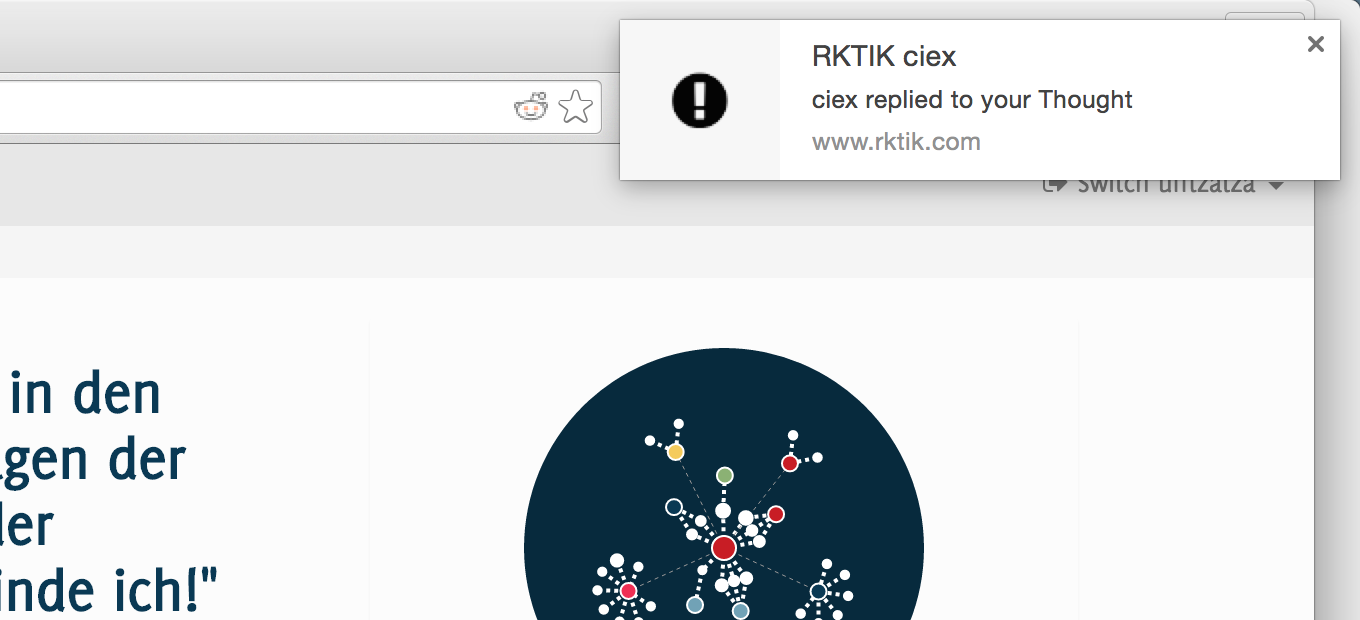
\includegraphics{img/desktop_notification.png}
\caption{Desktop notification indicating a new reply on a user's
thought}
\end{figure}

Notifications are direct messages from the system to individual users
and inform them about reactions to their thoughts, as well as other
relevant messages. They are relayed as desktop notifications and/or as
email messages. Email messages provide the further advantage of being a
way to contact users who are not visiting the site regularly.

Desktop notifications are displayed using the PNotify library
(\href{http://sciactive.github.io/pnotify/}{PNotify}), which can insert
notifications as HTML elements in web pages or as operating system
specific native UI elements outside the browser window, as specified in
the W3C recommendation \emph{Web Notifications} (see W3C (n.d.)). When
users first visit the Rktik website, they are prompted to allow
displaying web notifications. HTML based notifications are used if this
request is denied. Desktop notifications are relayed to the browser
using websockets. The javascript functions used for receiving and
displaying notifications are located in the
\texttt{glia/static/js/main.js} script.

Email notifications are delivered using the \emph{SendGrid} email
delivery service (\href{https://sendgrid.com/}{SendGrid website}). Using
this service ensures that all users can receive email notifications
reliably. While an email implementation integrated with the Rktik
service would be technically feasible, this approach would not guarantee
that messages pass spam filters of users' email providers. This
functionality is implemented in the \texttt{glia.web.helpers} module.

The user may opt out of email delivery entirely or set up specific rules
for the kind of emails they want to receive. These settings can be made
in the notifications view. This page is linked from the notifications
drop-down and from the footer section of all email notifications sent by
Rktik.

\hyperdef{}{improving-performance}{\section{Improving
Performance}\label{improving-performance}}

User satisfaction is related to a web site's performance (NIELSEN
(2012)). As the complex page layouts and \emph{hot} sorting used in
Rktik require significant server resources, keeping performance at a
satisfactory level is hard. As the development process of Rktik did not
define performance as a primary objective (see
\hyperref[methodology]{Methodology}), the neccessary adjustments are
even more difficult to make. Still, it was possible to increase
performance at the end of the development process by 1) using memcache
to reuse computed results and 2) optimizing database queries.

\textbf{Caching}

The memcache system is an in-memory key value store to hold computed
results for fast access. Entries in memcache persist until they are
overwritten, their expiry date is reached or they are deleted because
available memory is not sufficient for new entries. Rktik uses the
Flask-Cache library to access memcache
(\href{https://pypi.python.org/pypi/Flask-Cache/0.13.1}{Flask-Cache
0.13.1 website}). Caching is used if results 1) are changing
slowly\footnote{As an example, the frontpage graph structure is cached
  for one hour per persona as the frontpage changes slowly and omissions
  are not considered critical.} , 2) are expected to be reusable in the
near future, and 3) can be reliably invalidated once they change.

Cached data is invalidated by processes that change its contents. See
{[}Cached Information{]} for a list of cached functions and the
processes that trigger their invalidation. Cache contents are
automatically invalidated after an amount of time that ranges from
minutes to days.

\textbf{Database Query Optimization}

The SQLAlchemy library hides the complexity of accessing data stored and
linked across multiple tables. While this eases the development process
significantly, it can lead to inefficient patterns of database usage.
Specifically, the number of queries required to access data can be in a
linear relation to the number of items retrieved. Often, such queries
can be combined into a single query or a low number of queries by using
\emph{eager loading} techniques offered by SQLAlchemy (SQLAlchemy Autors
(n.d.)). Here, a \emph{JOIN} statement is issued to simultaneously load
related data from the database. Rktik is configured to utilize eager
loading 1) for specific queries, using the SQLAlchemy
\texttt{joinedload} option, and 2) for certain model properties in
general by specifying the option as a parameter in Nucleus' model
definitions.

\hyperdef{}{hosting-and-deployment}{\section{Hosting and
Deployment}\label{hosting-and-deployment}}

Rktik ist running on servers provided by the Heroku
platform-as-a-service (PAAS) \^{}{[}\href{https://www.heroku.com}{Heroku
website}). In contrast to traditional server environments, which need to
be manually configured for the services to be deployed, a PAAS offers
tools that automate many of these tasks. This includes deployment from a
Git repository, automatic installation of dependencies, a web interface
for installation and semi-automatic configuration of third-party
services (e.g.~email delivery, memcache, log analysis, etc.) and a
mechanism for simple and fast scaling of an application's resources in
the event of rising visitor traffic.

These capabilities allow developers to focus on programming instead of
the time-consuming configuration and maintenance of a server
environment. The downside of using Heroku is that their services come at
a comparatively high price. This downside is mitigated, as Heroku is
offering a free option for applications that require only little
resources as is the case for Rktik right now. However, if Rktik grows to
a larger userbase, it might become necessary to move to a different
hosting environment that offers a better cost-benefit ratio.

Rktik is installed in two separate Heroku environments for
\emph{testing} and \emph{production} use. The development process
consists of testing a new feature on a local development machine,
testing it in the testing environment and only then deploying it to the
production environment if no bugs are found (see
\hyperref[methodology]{Methodology}). The production environment has
been accessible to the general public since July 26th 2015.

Deployment to these environments is automated using the scripts
`push\_testing.py' and `push\_production.py' in the source code's root
folder. These scripts execute all tasks neccessary for deployment which
includes:

\begin{itemize}
\tightlist
\item
  Verifying that all changes to the Nucleus repository are committed in
  Git
\item
  Pushing the Nucleus repository to Github
\item
  Checking that all changes to the Glia repository are committed in Git
\item
  Pushing the Glia repository to the appropriate environment on Heroku.
  This step triggers the Heroku environment to automatically install all
  required dependencies.\footnote{Dependencies are defined in the file
    \texttt{requirements.txt} in the Glia project root folder}
\item
  Running database migration scripts in the Heroku environment
\end{itemize}

The script for deployment to the production environment additionally
merges all changes in the \emph{development branch} into a new commit on
the \emph{master branch} of the Glia repository (see
\hyperref[methodology]{Methodology}). Therefore, commits on the master
branch represent a history of deployments to the production environment
and can be seen as versions of the Glia application.

Rktik uses \emph{environment variables} to determine which environment
it is currently running in and to load an appropriate configuration.
There are differing configurations for the development, testing and
production environment. They differ in the passwords, secrets and
external services they specify, as well as the internet hostname they
set up for Rktik. Sensitive information such as passwords is not stored
in the source code repository, but loaded either from access-controlled
external files or environment variables.

The development and testing configurations additionally increase the
verbosity of log messages and provide interactive debugging in two ways:
1) a debugging console and interactive traceback embedded in Flask's
response when server errors occur during a request and 2) the Flask
DebugToolbar (Tellingen \& Individual Contributors (2015)), which
provides an interface for performance measurement, variable
introspection and other information as an optional web overlay for
successful requests.

All logging messages above the \emph{debug} severity level are also
forwarded to the Rktik engineering channel in the Slack web
service,\footnote{The \href{https://slack.com}{Slack web service}
  provides chat rooms which can be integrated with external web services}
which is not visible to the public. This allows monitoring of errors in
Rktik from a mobile phone or any computer with an internet connection.

\chapter{Evaluation and Discussion}\label{evaluation-and-discussion}

Rktik is an evolution of the Souma prototype, introducing changes in
some areas and taking a completely different approach in others. In this
section I will reflect critically on how Rktik measures up to
expectations set at the onset of its implementation and underline these
findings with data from quantitative usage metrics.

\section{Personal Evaluation}\label{personal-evaluation}

The goals of \textbf{completeness}, \textbf{feasibility} and
\textbf{maintainability}, as defined in section
\hyperref[methodology]{Methodology}, have been reached by the
implementation described in this document. Development of the necessary
features for \emph{publishing} and \emph{discussing} content using
personas and movements have been built, and an appropriate environment
for the operation of Rktik has been configured. While these initial
goals are important, other aspects of Rktik have shown shortcomings in
the course of development and testing. In this areas I have identified
three aspects based on my own experiences and informal feedback received
from acquaintances.

\begin{enumerate}
\def\labelenumi{\arabic{enumi}.}
\item
  Some of the concepts used in Rktik, such as the distinction between a
  private mindspace and a public blog or the concept of movements, are
  hard to understand for new users. This problem should be approached by
  building a tutorial, which explains core mechanics and concepts. It
  can be presented after signup and should be conceived for both new
  users with an account and potential, but unregistered users.
\item
  As described in the section \hyperref[improving-performance]{Improving
  Performance}, the site's speed is still too low for web user's
  expectations. This can be improved by setting up periodically running
  background processes that precompute database queries and store them
  in memcache. Site performance could also be improved significantly by
  moving Rktik to more powerful servers, which however increases the
  costs of running the service.
\item
  Rktik features interesting content that is regularly updated. Users
  who have signed up for an account but do not visit the site regularly
  could benefit from this through a periodic email newsletter. Each
  edition of the newsletter may feature the most interesting content on
  Rktik as measured by votes received on thoughts.
\end{enumerate}

\section{Usage Metrics}\label{usage-metrics}

Usage metrics have been collected anonymously using the
Amplitude\footnote{\href{https://amplitude.com/}{Amplitude website}} and
Google Analytics\footnote{\href{https://www.google.com/analytics/}{Google
  Analytics website}} services. These are external services which
receive usage data via short Javascript scripts embedded in every served
page. As I consider this usage data \emph{personal information}, it is
collected anonymously. While Google Analytics tracks information about
page requests, Amplitude tracks specific, manually defined events in a
user's interaction with the site.

Google Analytics data is included since making rktik.com accessible to
the public on July 26th 2015 until October 2nd 2015 for a total of 68
days. Amplitude data is included from August 8th 2015 until October 2nd
2015 for a total of 55 days. This difference exists because I only found
out about Amplitude when measurement had already begun.

Google Analytics and Amplitude collect extensive amounts of information.
As a complete analysis of the data would go beyond the scope of this
thesis, I have focussed on four kinds of measurement: 1) The total
number of usage sessions, 2) the number of users per week, 3) the number
of users who have used specific features in a given week, and 4) the
number of thoughts and votes created. These metrics were chosen because
they reflect the total amount of usage, as well as the relative
popularity of specific features.

For the purpose of this evaluation, a \emph{user} is defined as a web
browser used to access Rktik. In contrast to the definition given in the
\hyperref[terminology]{Terminology}, this does not discriminate between
users with an Rktik user account and anonymous users. While it is
possible that a person uses more than one web browser to access Rktik,
this is not reflected in measurements. Usage assessment using Google
Analytics and Amplitude relies on Javascript scripts embedded in the
site. If a user has blocked these scripts or disabled Javascript
altogether in their browser, their usage is not recorded.

\subsection{Usage sessions}\label{usage-sessions}

The number of sessions was assessed using Google Analytics. A session is
defined as a group of interactions between a user and the website that
takes place within 30 minutes or until midnight (Google (n.d.)). A total
of 825 sessions were started, most of which took place in the first
weeks of operation. The number of sessions following the first two weeks
of operation may have been higher if Rktik had been promoted more
extensively. This process was stalled due to the currently high access
times described in \hyperref[improving-performance]{Improving
Performance}.

\begin{figure}[htbp]
\centering
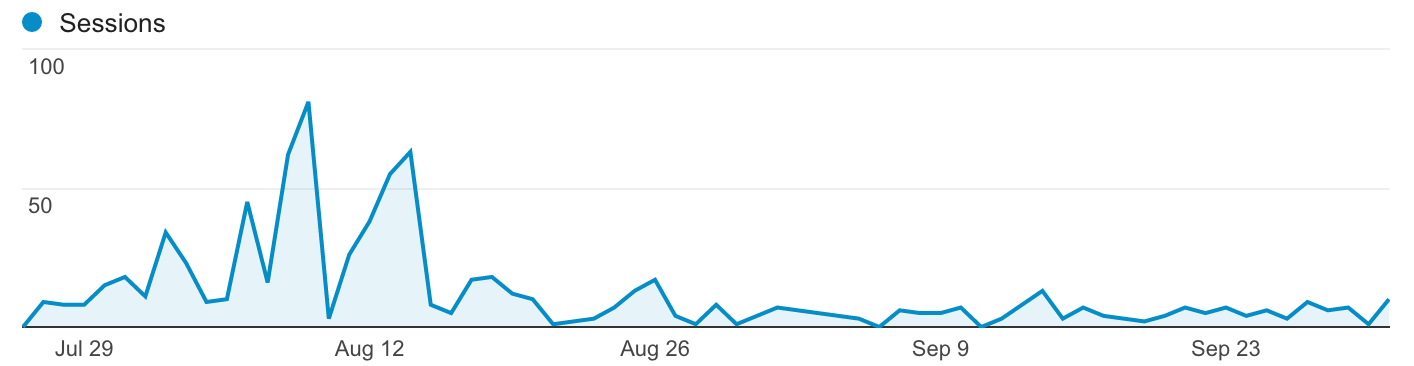
\includegraphics{img/eval_sessions.png}
\caption{Number of sessions}
\end{figure}

\subsection{Users per week}\label{users-per-week}

The number of users per week was assessed using Amplitude. The count
rises from two users in the first week of measurement to seven users in
the third and fourth week. It takes a plunge to three users and then
rises from week to week up to a maximum of 17 users in the 9th week of
operation.

\begin{figure}[htbp]
\centering
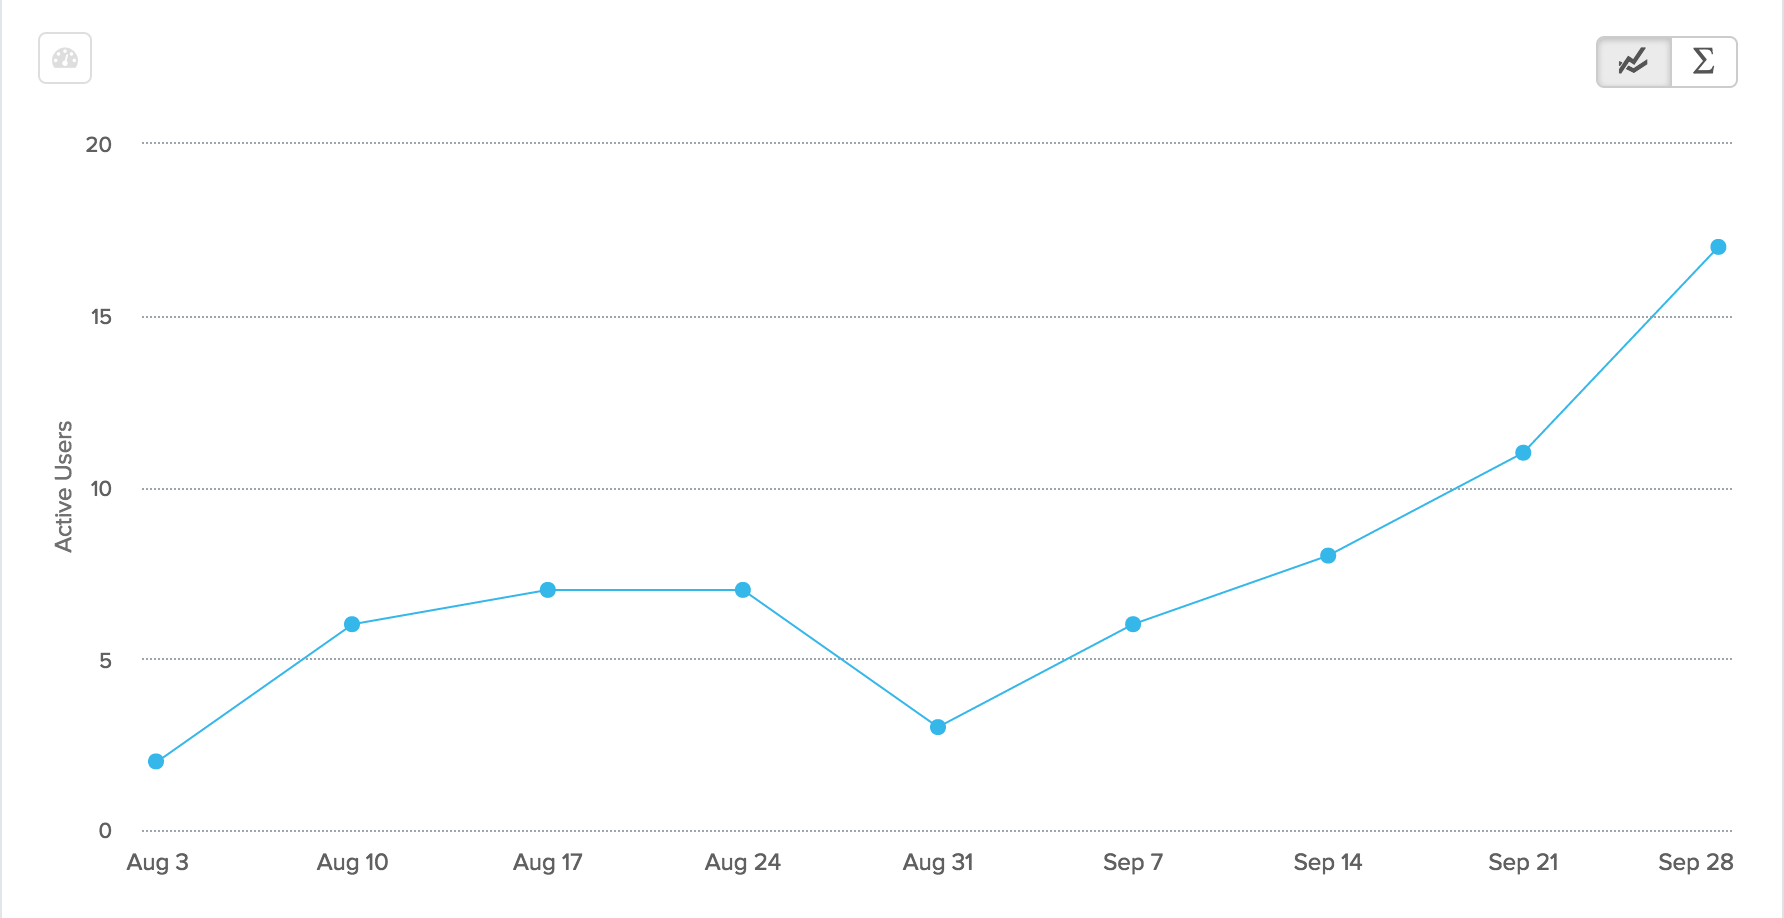
\includegraphics{img/eval_weekly_users.png}
\caption{Number of weekly users}
\end{figure}

\subsection{Usage of features}\label{usage-of-features}

The number of users who have used specific features at least once in a
given week was assessed using Amplitude. A count was recorded by firing
an Amplitude callback when a user triggered the user interface control
associated with the measured action. In the following I list the
assessed metrics and events used to measure them and describe the
resulting measurement data.

\subsubsection{Creating a thought}\label{creating-a-thought}

Evaluated: 1) submitting the inline form for creating a thought 2)
submitting the form on the dedicated \emph{create thought} view

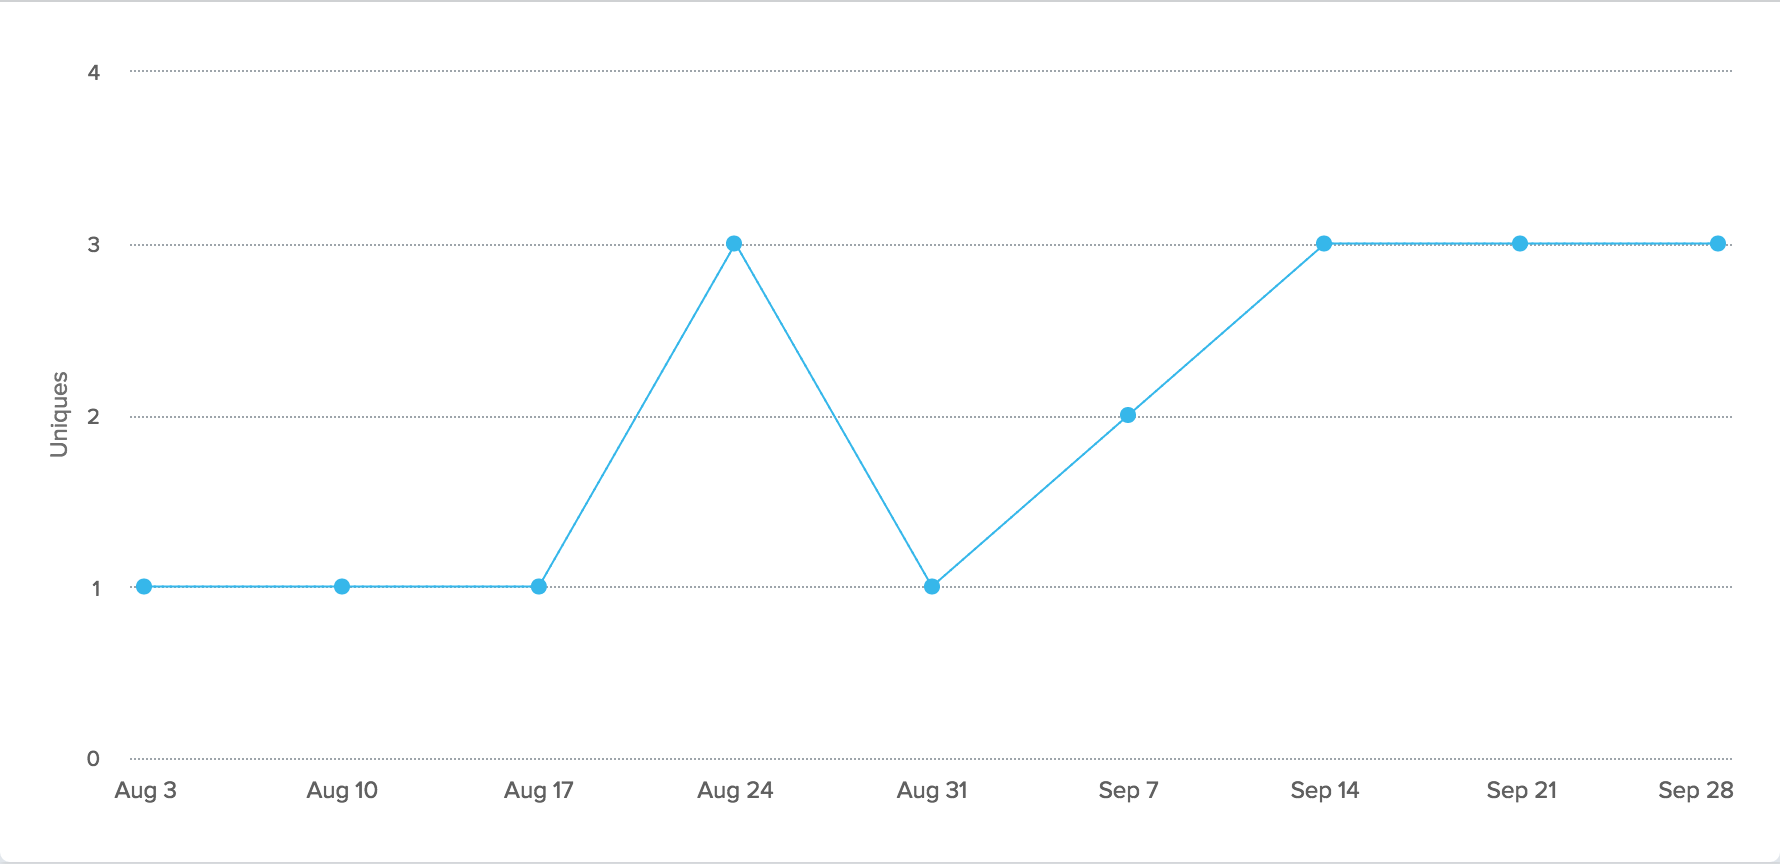
\includegraphics{img/eval_create_thought.png}\\
 Over the duration of measurement the number of users who create
thoughts in a given week varies between one and three. The maximum
number of three users was first reached in the fourth week of
measurement and in the last three weeks of measurement there were never
less than three users creating thoughts. Only a small amount of total
users registered an account on Rktik. Out of those registered users,
only a small amount actively created content.

\subsubsection{Editing a thought}\label{editing-a-thought}

Evaluated: Submitting the form for editing a thought in the \emph{edit
thought} view.

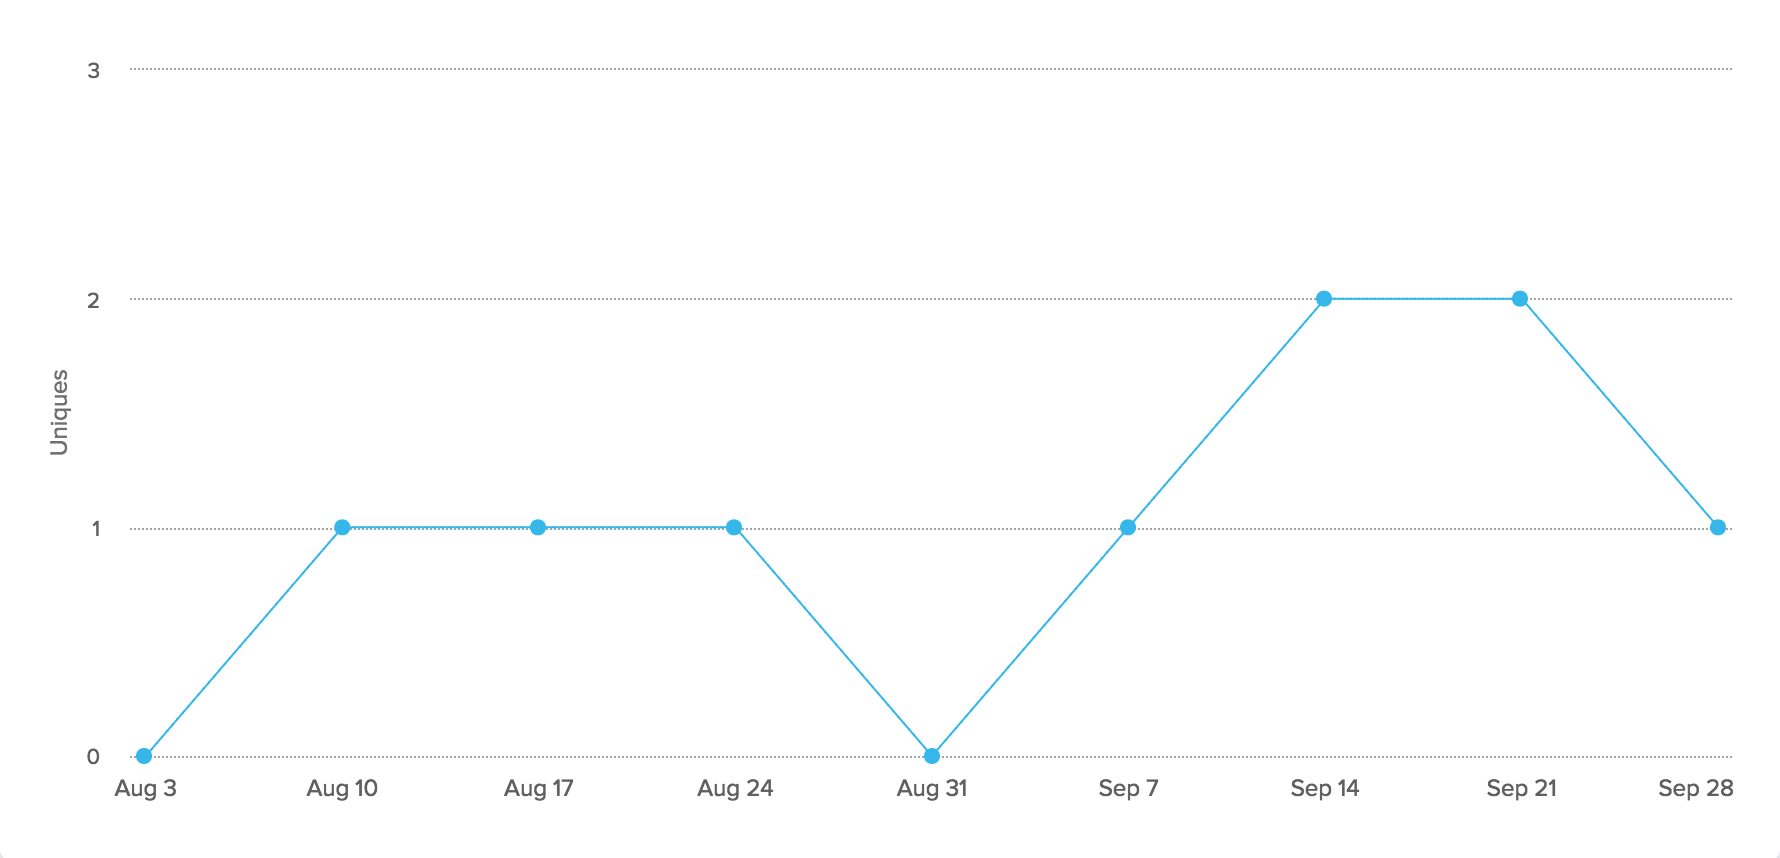
\includegraphics{img/eval_edit_thought.png}\\
 The number of users who edited thoughts in a given week varies between
zero and two. Unexpectedly, this number is not much lower in a given
week than the number of users who created thoughts. This means that most
users who create thoughts also edit them.

\subsubsection{Clicking the graph
visualization}\label{clicking-the-graph-visualization}

Evaluated: Completed mouse click in any part of the frontpage graph
visualization (see \href{img/graph.png}{Frontpage Graph Visualization}).

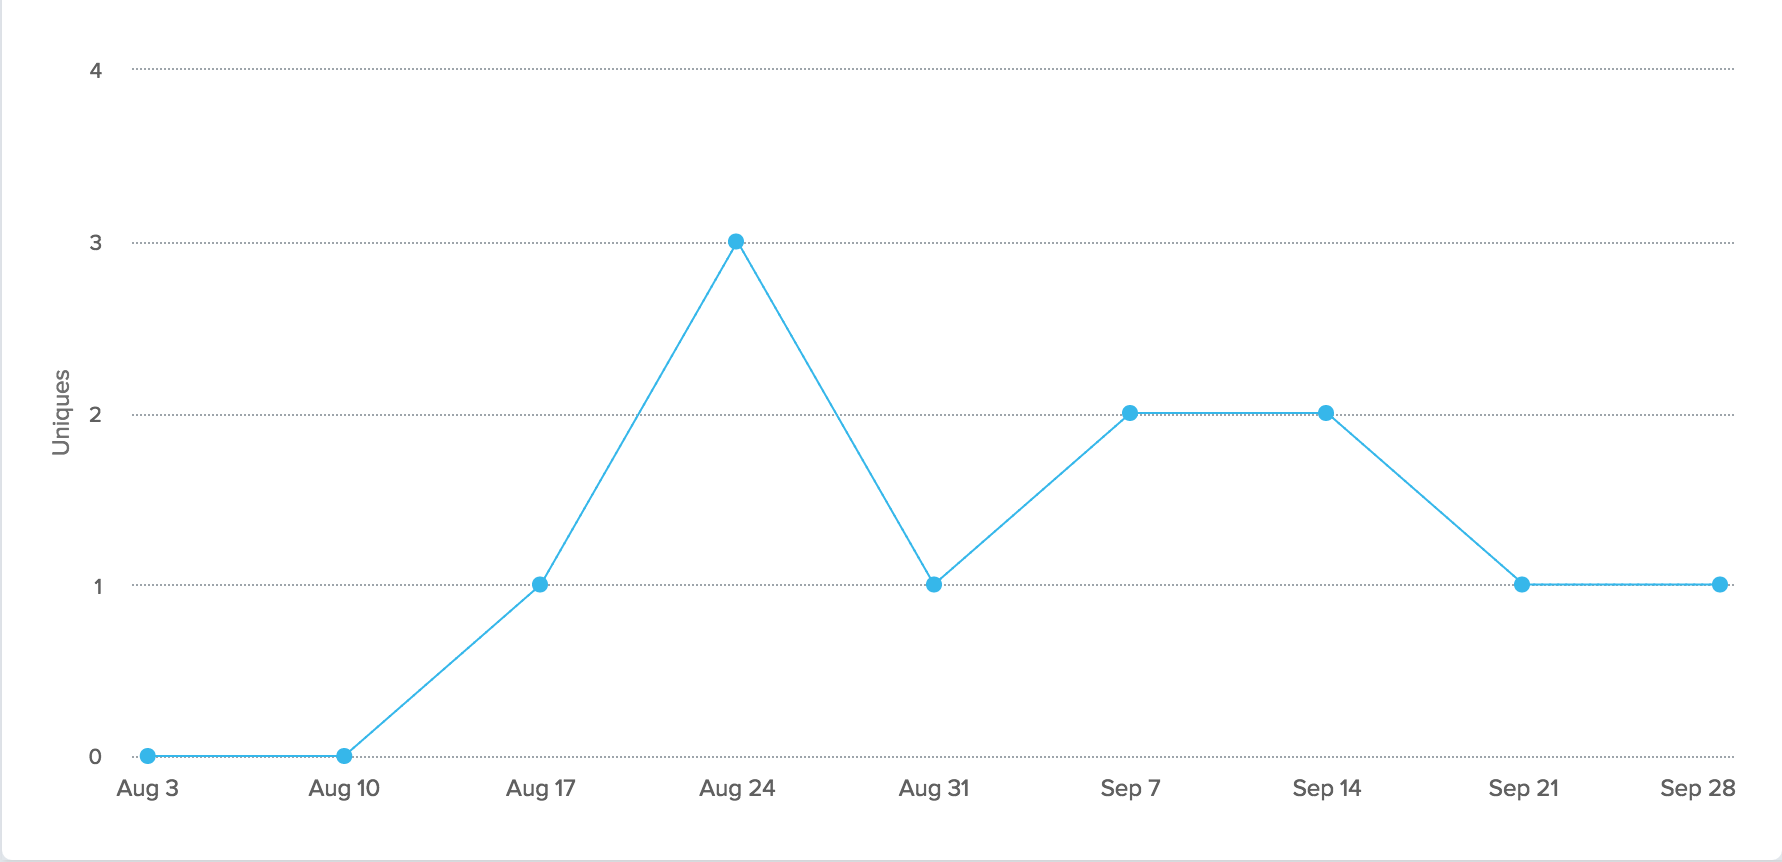
\includegraphics{img/eval_click_graph.png}\\
 The number of users who clicked on the frontpage graph visualization in
a given week varies between a minimum of zero users in the first two
weeks and a maximum of three users in the fourth week of measurement. As
the number of clicks does not return to the maximum of three users and
rests at one user per week in the last two weeks of measurement, it may
be assumed that users try this feature only once and do not return to it
later.

\subsubsection{Follow or unfollow a
blog}\label{follow-or-unfollow-a-blog}

Evaluated: Click on the \emph{follow} or \emph{unfollow} buttons located
in movement or personal blogs and in movement mindspaces.

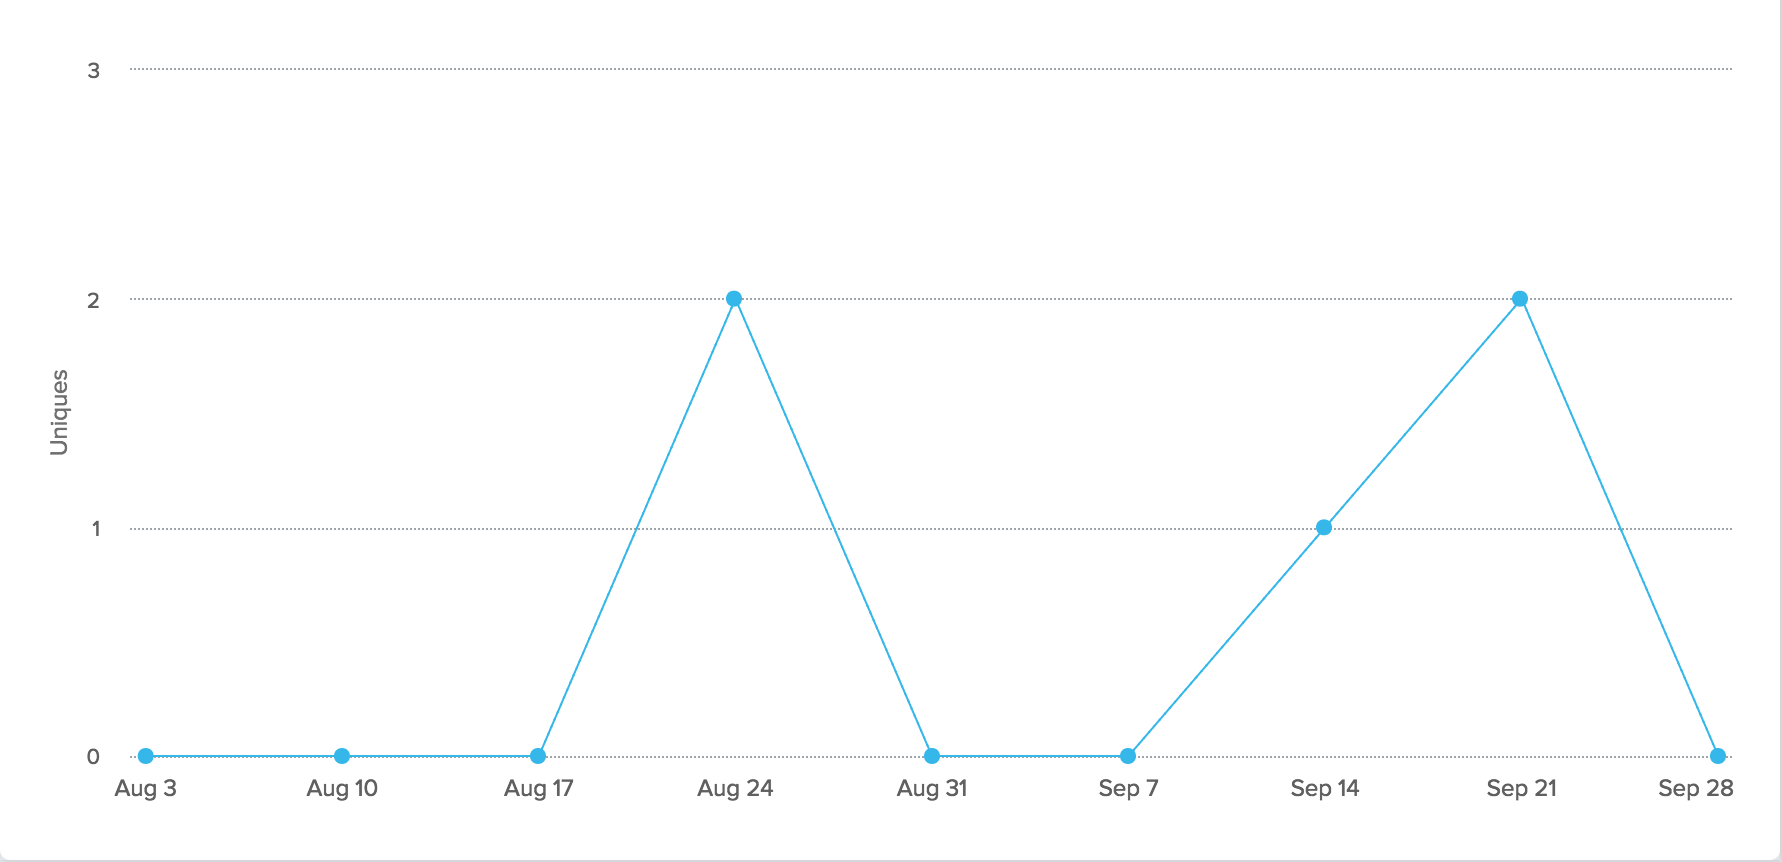
\includegraphics{img/eval_follow.png}\\
 The number of users who follow or unfollow blogs lies between zero and
two users over the course of measurement. This number is unexpectedly
low in relation to the total number of active users, especially towards
the end of the measurement. This may indicate that users do not
understand the purpose of this feature well enough. Educating users
about the possibility of controlling the contents of their frontpage by
following or unfollowing blogs may lead to a better user experience for
them.

\subsubsection{Toggle membership in a
movement}\label{toggle-membership-in-a-movement}

Evaluated: Click on the \emph{Join movement} or \emph{Leave movement}
buttons located in movement blogs and movement mindspaces.

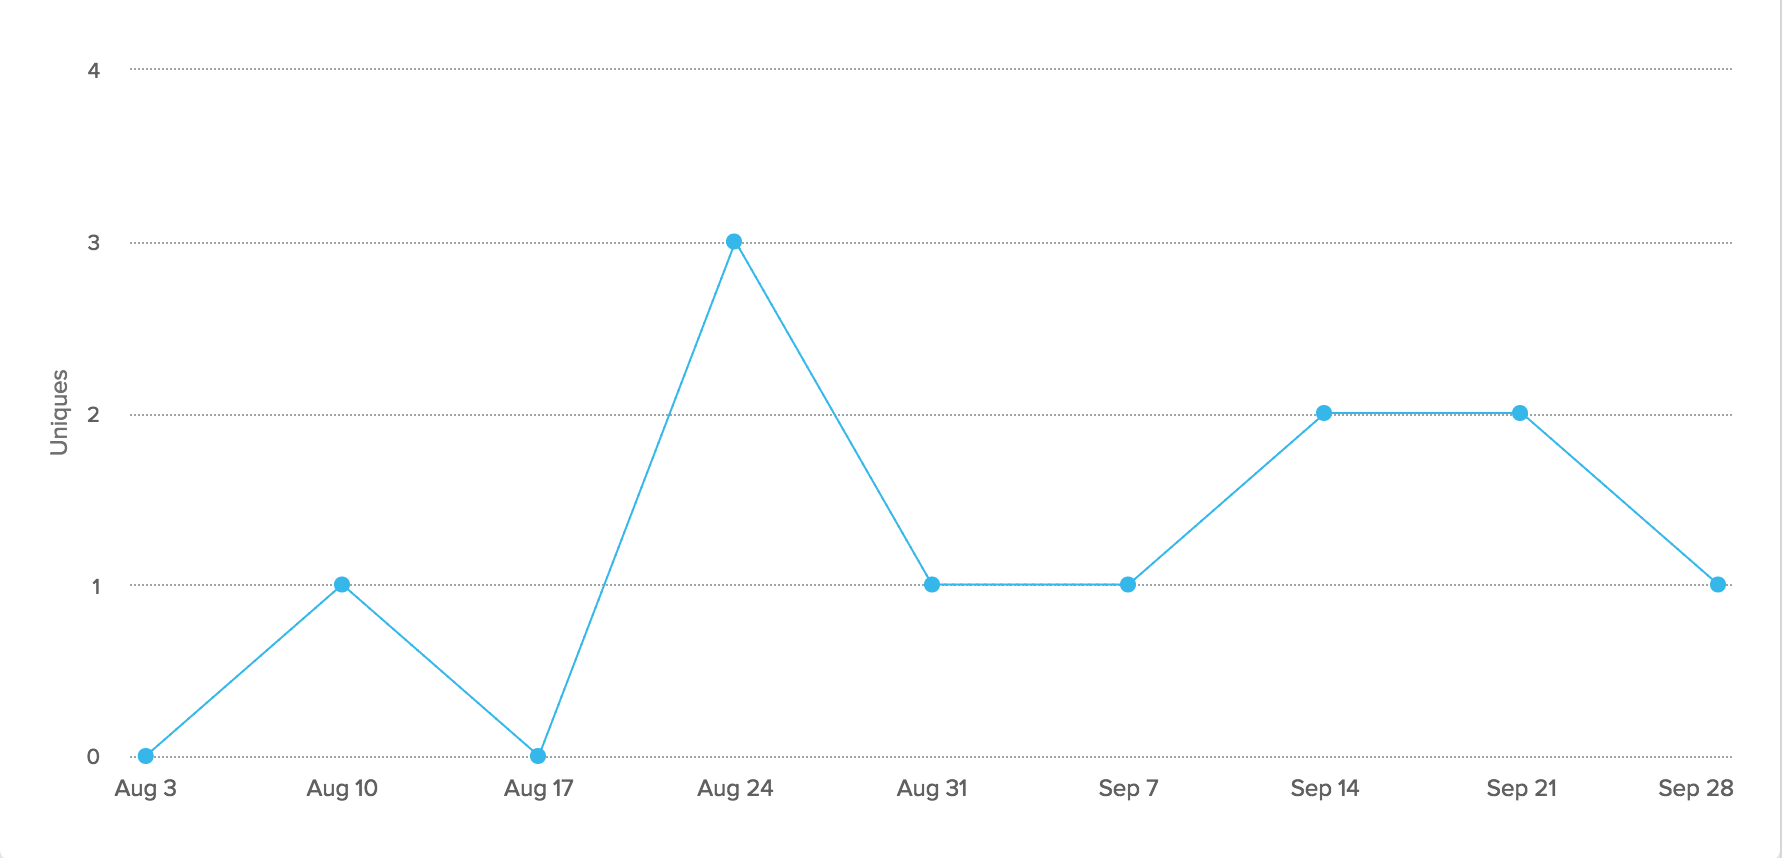
\includegraphics{img/eval_membership.png}\\
 The number of users who toggled their membership in movements is either
one or two in the first three weeks, reaches a maximum of three users in
the fourth week and varies between one and two users for the remainder
of the measurement. Similar to the number of users who follow or
unfollow blogs, this number is unexpectedly low and suggests that users
do not understand the benefits of controlling their membership in
movements well enough.

\subsubsection{Accessing the notebook
view}\label{accessing-the-notebook-view}

Evaluated: Loading the notebook view

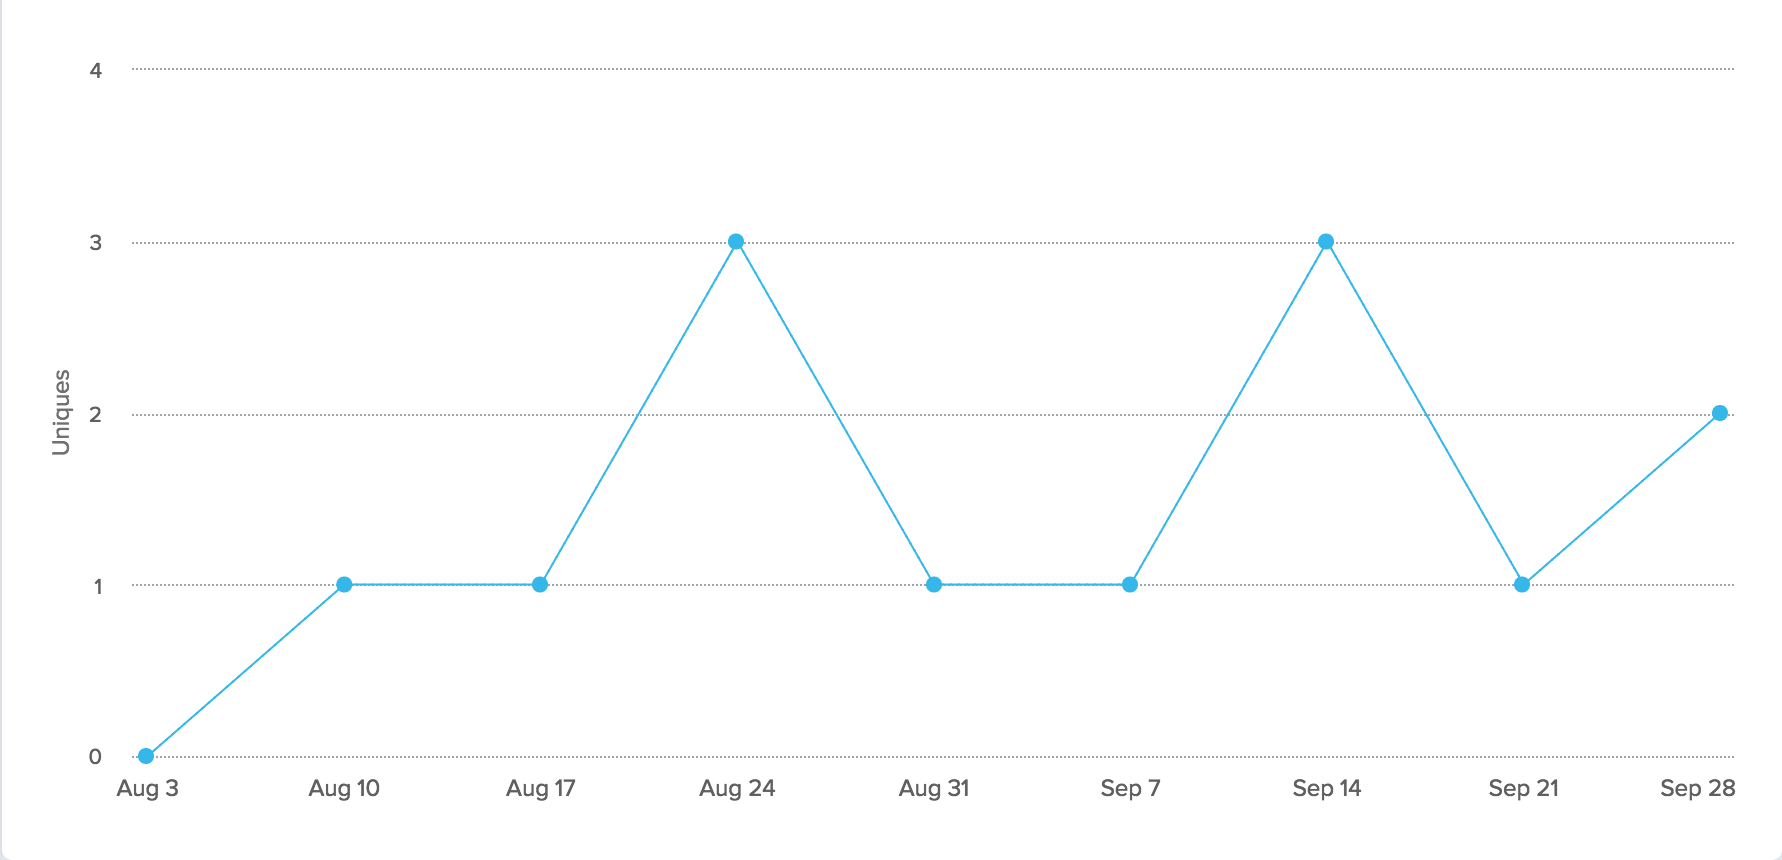
\includegraphics{img/eval_notebook.png}\\
 The number of users who view their notebook is zero in the first week
and varies between one and three users for the remainder of the
measurement. The feature was not used in the first week because it was
only activated in the second week of measurement. Engagement with this
feature may be higher if it was more integrated with other features of
the site. Right now, the flow of data in and out of the notebook is
achieved via the \emph{repost} functionality. This mechanism may be
poorly understood by users which could be helped by a more comprehensive
tutorial for new users.

\subsubsection{Toggling a vote}\label{toggling-a-vote}

Evaluated: Completed mouse click on a vote button

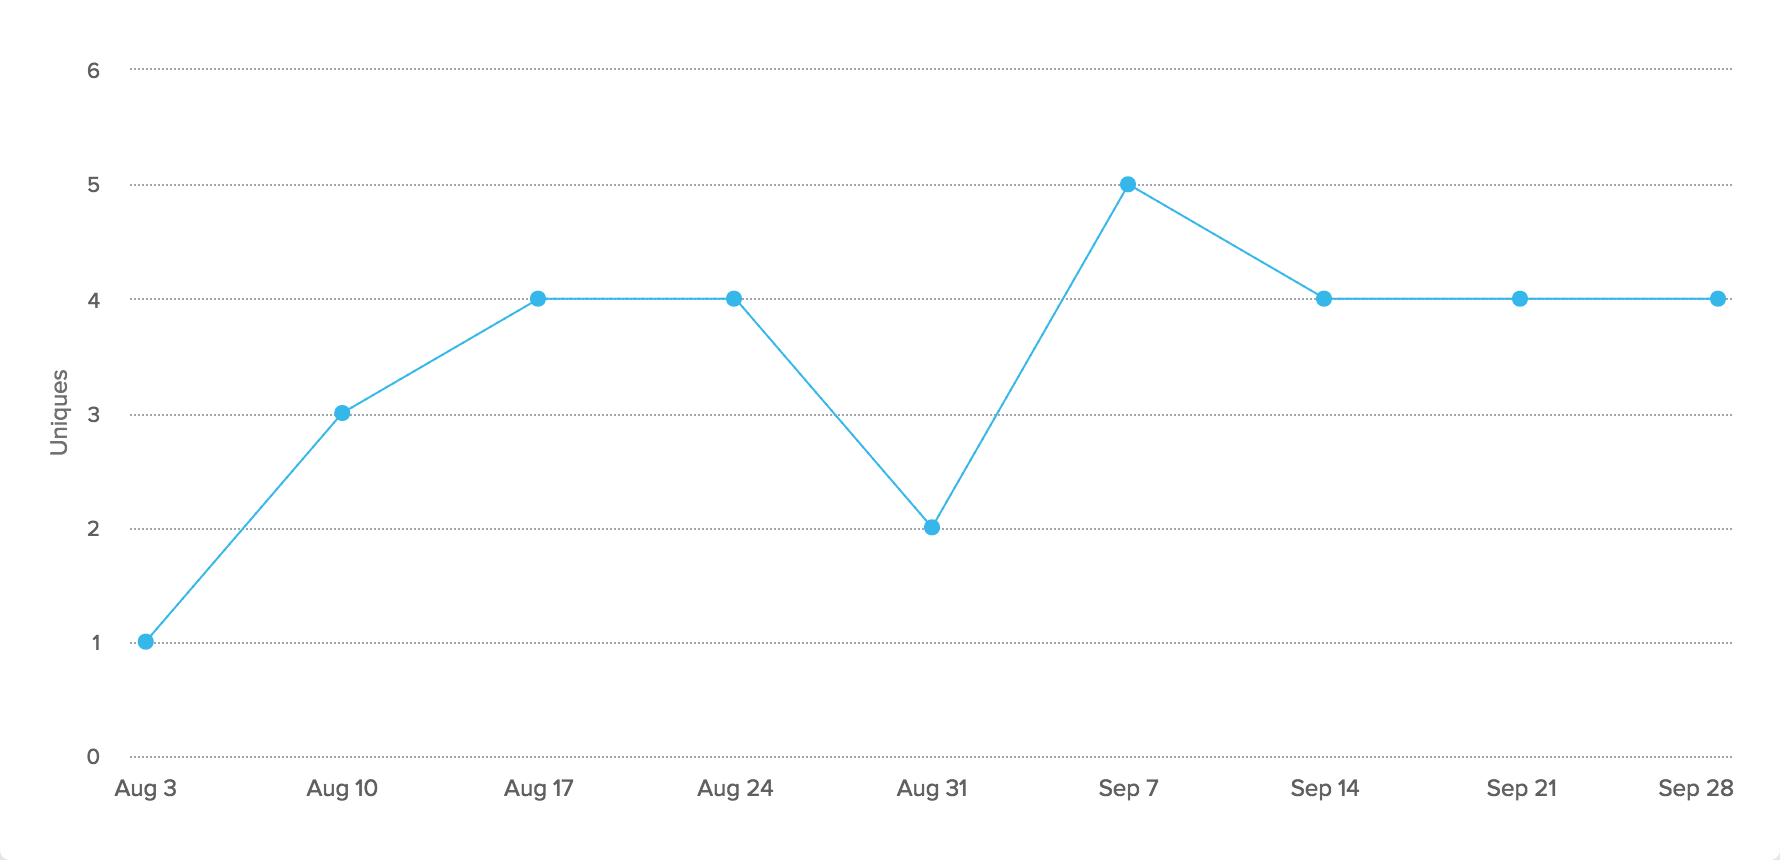
\includegraphics{img/eval_vote.png}\\
 The number of users who cast votes rose from one in the first week to
four in the third week and remained at this level except for the 5th and
6th weeks, where two and five users engaged with the feature
respectively. This feature was the most popular in this comparison,
which confirms its nature as a low-barrier way of engaging with content
in Rktik.

The evaluation of user metrics shows how different features are accepted
by users. Although the explanatory power of these observations is
limited due to the low number of users, some interesting observations
include the fact that a high number of users edit their posts and that
very few users change their blog subscriptions or membership in
movements. Especially the latter fact highlights the need for a tutorial
that will guide new users through the features of Rktik. The continued
observation of these measurements will allow a focussed development of
Rktik in the future.

\hyperdef{}{movement-agency}{\section{Movement
Agency}\label{movement-agency}}

Rktik communicates to its users that movements have agency. This is
established by attributing actions taken by its members to the movement
itself, once they are confirmed by a certain number of other members. As
described in \hyperref[movements]{Movements} this process 1) guards
members' privacy and 2) may establish stronger cohesion between movement
members.

While this concept may be applicable to a wide range of actions, Rktik's
current implementation only supports attributing authorship of a thought
to a movement (see \hyperref[promoting-content]{Promoting Content}). In
this section I will present three options for other actions that may be
attributed to a movement's agency through building consensus among its
members.

Planning and voting of any such collective actions may be conducted
using a novel interface control which allows members to 1) identify the
proposed action, 2) propose changes, and 3) vote on its implementation.
This control should be designed for the control of all action types to
simplify the process for inexperienced users.

\textbf{Events}

A movement member may propose an event in the movement mindspace. An
event consists of a title, location, date, time and privacy setting
(visible only for members or for all users) and can be implemented as an
attachment type. Other members can discuss the events and propose
changes to be made by the author in order to gain their consensus, and
thus the necessary votes for making the event official. Finally, members
vote on the event. If this shows that consensus is reached, the movement
displays the event prominently in the movement mindspace or movement
blog, depending on the event's privacy settings. The final event posting
is attributed to the movement and not its original author. This mechanic
would allow movement members to organize collective action outside of
Rktik's online context.

\textbf{Public chat}

A movement's (public) blog may contain a chat module, which non-members
can use to converse with the movement as a whole. Messages entered in
this chat would be displayed in the movement mindspace for members to
see. Members can then propose answers and other members can confirm
these by voting on them. The non-member who posted the original message
into the movement chat would then be shown the answer attributed to the
movement as a whole.

\textbf{Creating thoughts in other parts of the site}

Members may propose a thought to be posted with attribution to the
movement in another part of Rktik. This could be a personal message to a
persona, a reply to any thought not in the movement itself or as a
message in the public chat of another movement (as described above).
Changes to the proposed thought may be discussed by members beforehand
as described for \emph{events} and \emph{public chat} .

\hyperdef{}{external-clients}{\section{External
Clients}\label{external-clients}}

Rktik is the successor to Souma, which is a prototype for a decentral
social network as described in
\hyperref[problem-privacy-and-identity]{Problem: Privacy and Identity}.
While Rktik is not built as a decentral system, its design allows a
future extension with such functionality. Such an extension would entail
two parts: 1) a publicly accessible API for Rktik's Nucleus backend, and
2) a local client application that connects to this API. Using a local
client makes a new usage pattern possible in which a private movement's
internal data is only stored in encrypted form on the server. Encrypted
information about members' activity would be distributed among them via
the API. Information would only be made available in unencrypted form on
the rktik.com website once members have decided on a collective action.
In this section I will outline the components necessary to build this
extension based on the design implemented by Souma (see Ahrend (2015)).

\textbf{API for Rktik's Nucleus module}

An API is an interface between two separate pieces of software. JSON and
HTTP REST APIs have emerged as de facto standards in web infrastructure
(CITE). The API will serialise ORM models into JSON representations that
are encrypted, signed and wrapped in a second layer JSON representation
for transfer.

{[}TODO: Diagramm{]}

The API will be designed primarily for a client that is installed on a
user's computer, but it may also be used for third party services built
on data published by Rktik. Usage scenarios include clients for mobile
devices or third-party websites that interact with Rktik.

\textbf{Local client application}

An external client uses the aforementioned API to exchange data with
Rktik's server-based Nucleus backend and provides its own user interface
on the user's local machine. The implementation of this user interface
may reuse most of the code from Rktik's Glia web server to locally serve
a version of the site via a loopback connection.\footnote{TODO: Footnote
  about loopback connections} Differences in implementation would be
expected mostly from 1) code to access the API, and 2) performance
optimizations for personal computers.

While such an implementation of an external client would not technically
constitute peer to peer data transfer, as data is still transferred
using a server, it would bring all of its advantages with it:
End-to-end-encryption of data ensures that the contained
\emph{information} is only available at the endpoints of communications.
At the same time, the server-based infrastructure would 1) ensure that
data is available, even when no local machines are online, and 2)
increase synchronization speeds significantly by profiting off the
superior connection speeds available in data centers.

\part*{Bibliography} \manualmark
\markboth{\spacedlowsmallcaps{\bibname}}{\spacedlowsmallcaps{\bibname}}
\refstepcounter{dummy}
\addtocontents{toc}{\protect\vspace{\beforebibskip}}
\addcontentsline{toc}{chapter}{\tocEntry{\bibname}}

\chapter*{\bibname}

\hyperdef{}{ref-Ahrend2015}{\label{ref-Ahrend2015}}
Ahrend, V. (2015). Implementation. In L. Berov, A. Jamneshan, \& L.
Wjatscheslaw (Eds.), \emph{From a humanistic reconstruction of social
networks to souma} (pp. 95--108). Osnabrück: Not published.

\hyperdef{}{ref-Boyd2012}{\label{ref-Boyd2012}}
Boyd, D. (2012). The politics of ``real names''. \emph{Communications of
the ACM}, \emph{55}(8), 29.
\href{http://doi.org/10.1145/2240236.2240247}{doi:10.1145/2240236.2240247}

\hyperdef{}{ref-Facebooka}{\label{ref-Facebooka}}
Facebook. (n.d.-a). Can I have more than one username for my Page or
profile? Retrieved from
\url{https://www.facebook.com/help/154889281245103}

\hyperdef{}{ref-Facebook}{\label{ref-Facebook}}
Facebook. (n.d.-b). Facebook Company Info. Retrieved from
\url{http://newsroom.fb.com/company-info/}

\hyperdef{}{ref-Google}{\label{ref-Google}}
Google. (n.d.). How a Session is defined in Analytics. Retrieved from
\url{https://support.google.com/analytics/answer/2731565?hl=en}

\hyperdef{}{ref-Gruber2004}{\label{ref-Gruber2004}}
Gruber, J. (2004). Markdown. Retrieved from
\url{http://daringfireball.net/projects/markdown/}

\hyperdef{}{ref-NIELSEN2012}{\label{ref-NIELSEN2012}}
NIELSEN, J. (2012). User Satisfaction vs. Performance Metrics. Retrieved
from
\url{http://www.nngroup.com/articles/satisfaction-vs-performance-metrics/}

\hyperdef{}{ref-Radicati2011}{\label{ref-Radicati2011}}
Radicati, S., \& Hoang, Q. (2011). Email statistics report, 2011-2015.
\emph{Retrieved May}, \emph{44}(0), 0--3. Retrieved from
\url{http://scholar.google.com/scholar?hl=en\{/\&\}btnG=Search\{/\&\}q=intitle:Email+Statistics+Report+,+2011-2015\{/\#\}0}

\hyperdef{}{ref-Reddita}{\label{ref-Reddita}}
Reddit. (n.d.-a). About reddit. Retrieved from
\url{https://www.reddit.com/about/}

\hyperdef{}{ref-Reddit.com}{\label{ref-Reddit.com}}
Reddit. (n.d.-b). Reddit FAQ: Is it okay to create multiple accounts?
Retrieved from
\url{https://www.reddit.com/wiki/faq\{/\#\}wiki\{/_\}is\{/_\}it\{/_\}okay\{/_\}to\{/_\}create\{/_\}multiple\{/_\}accounts.3F}

\hyperdef{}{ref-Salihefendic2010}{\label{ref-Salihefendic2010}}
Salihefendic, A. (2010). How Hacker News ranking algorithm works.
Retrieved from \url{http://amix.dk/blog/post/19574}

\hyperdef{}{ref-SQLAlchemyAutors}{\label{ref-SQLAlchemyAutors}}
SQLAlchemy Autors. (n.d.). Relationship Loading Techniques. Retrieved
from
\url{http://docs.sqlalchemy.org/en/rel\{/_\}0\{/_\}8/orm/loading.html}

\hyperdef{}{ref-VanTellingen2015}{\label{ref-VanTellingen2015}}
Tellingen, M. van, \& Individual Contributors. (2015). Flask
DebugToolbar. Retrieved from
\url{https://flask-debugtoolbar.readthedocs.org/en/latest/}

\hyperdef{}{ref-W3C}{\label{ref-W3C}}
W3C. (n.d.). Web Notifications (W3C Proposed Recommendation). Retrieved
from \url{http://www.w3.org/TR/2015/PR-notifications-20150910/}

\appendix

\part*{Appendix}

\section{API Specification}\label{api-specification}

API Specification documents

\section{Rights Management}\label{rights-management}

This table show which users/personas are allowed to make changes to
specific models.

Rights Management for Mindsets

~~~~~~Mindset \textbar{} Creating \textbar{} Updating \textbar{}
Deleting

Personal Mindspace --- Persona --- Personal Blog --- Persona ---
Movement Mindspace Members --- Author, Admin --- Movement Blog
Automatic* --- Admin --- Dialogue Members --- Author ---

\begin{verbatim}
* see section ___ on auto-promotion from movement mindspaces to blogs
\end{verbatim}

\section{Cached Information}\label{cached-information}

This section gives an overview of values cached using memcache as
described in section {[}Improving Performance{]}.

Methods: * Persona.attention * Persona.conversation\_list (invalidated
by Thought.create\_from\_input) * Persona.frontpage\_sources
(invalidated by Persona.toggle\_following,
Persona.toggle\_movement\_membership) * Persona.movements (invalidated
by Persona.toggle\_movement\_membership) * Persona.repost\_mindsets
(invalidated by Persona.toggle\_movement\_membership) *
Persona.suggested\_movements

\begin{itemize}
\item
  Movement.attention
\item
  Movement.member\_count (invalidated by
  Persona.toggle\_movement\_membership)
\item
  Movement.mindspace\_top\_thought (invalidated by
  Thought.toggle\_upvote)
\item
  Movement.top\_movements
\item
  Thought.top\_thought (invalidated by Thought.create\_from\_input)
\item
  Thought.upvote\_count (invalidated by Thought.toggle\_upvote)
\item
  Thought.iframe\_url
\end{itemize}

Additional: * Recent thoughts helper Nucleus.helpers.recent\_thoughts
(invalidated by Thought.create\_from\_input) * ``Percept'' template
macro * Frontpage graph visualization * Async chat view

\section{Usage Metrics}\label{usage-metrics}

\subsection{Amplitude}\label{amplitude}

\subsection{Google Analytics}\label{google-analytics}

\section{Source Code}\label{source-code}


\end{document}
